% Capítulos personalizados
\makeatletter
\renewcommand\chapter[1]{%
    \clearpage
    \thispagestyle{empty}
    \phantomsection
    \refstepcounter{chapter}% Actualiza y vincula
    \addcontentsline{toc}{chapter}{#1}%
    \vspace*{\fill}
    \begin{center}
        \normalfont\LARGE\bfseries #1
    \end{center}
    \vspace{\fill}
    \clearpage
    \setcounter{section}{0}
}
\makeatother

% Numeración de secciones en letras
\renewcommand\thesection{\Alph{section}}

% Secciones personalizadas
\makeatletter
\renewcommand\section[1]{%
    \phantomsection
    \refstepcounter{section}%
    \addcontentsline{toc}{section}{\protect\numberline{\thesection}#1}%
    {\normalfont\Large\bfseries \thesection. #1}%
}
\makeatother

\chapter{ANEXOS}

\begin{landscape}
\section{Matriz de consistencia}
%\addcontentsline{toc}{chapter}{ANEXOS}
%\textbf{\Large{ANEXOS}}\\
%\addcontentsline{toc}{section}{A. Matriz de consistencia}
%\textbf{A. Matriz de consistencia}
\begin{table}[h!]
\centering
%\caption{Matriz de Consistencia}
\footnotesize % Reduce el tamaño de la fuente para que quepa mejor
\begin{tabular}{|p{4.5cm}|p{4.5cm}|p{4.5cm}|p{3cm}|p{4.2cm}|}
\hline
\multicolumn{1}{|c|}{\textbf{Problemas}}  & \multicolumn{1}{c|}{\textbf{Objetivos}}  & \multicolumn{1}{c|}{\textbf{Hipótesis}} & \multicolumn{1}{c|}{\textbf{Variables}}   & \multicolumn{1}{c|}{\textbf{Metodología}} \\ \hline
\multicolumn{3}{|c|}{\textbf{General}}                               & \textbf{Dependientes}  & \multirow{4}{=}{
\begin{minipage}{4.2cm}
\justify
$\circ$ \textbf{Tipo:} Aplicado \\
$\circ$ \textbf{Enfoque:} Cuantitativo \\
$\circ$ \textbf{Alcance:} Descriptivo correlacional - Explicativo \\
$\circ$ \textbf{Diseño:} Retrospectivo longitudinal no experimental \\
$\circ$ \textbf{Población:} Productos de almacén. \\
$\circ$ \textbf{Población de estudio:} Productos clasificados mediante (ABC).\\
$\circ$ \textbf{Técnica de recolección de datos:} Revisión documental y/o datos secundarios. \\
$\circ$ \textbf{Instrumento de recolección de datos:} Boletas, ordenes de compra, KARDEX, cotizaciones. \\
$\circ$ \textbf{Método de análisis de datos:} Recopilación de datos en un archivo \textsl{.xlsx}, procesamiento y análisis de datos en el lenguaje de programación R mediante el entorno de desarrollo integrado RStudio.
\end{minipage}
} \\ \cline{1-4}
\multicolumn{1}{|p{4.5cm}|}{¿Cómo implementar los modelos de inventarios para optimizar el control de almacén del centro de salud integral La Fuente del Cusco durante el año 2024?} & \multicolumn{1}{p{4.5cm}|}{Implementar los modelos de inventarios para optimizar el control de almacén del centro de salud integral La Fuente del Cusco durante el año 2024.} & El control de almacén del centro de salud integral La Fuente del Cusco se optimizará mediante la aplicación de los modelos de inventarios. & 
    \vspace{0.2cm}
    $\circ$ Cantidad de pedido óptimo\vspace{0.2cm}

    $\circ$ Tiempo de pedido óptimo\vspace{0.2cm}
  &                       \\ \cline{1-4}
\multicolumn{3}{|c|}{\textbf{Específicos}}                               & \textbf{Independientes} &  \\ \cline{1-4}
\multicolumn{1}{|p{4.5cm}|}{
    $\circ$ ¿Cuáles son los productos más demandados y/o costosos en el centro de salud integral La Fuente del Cusco?\vspace{0.2cm}

    $\circ$ ¿Qué modelo de inventarios se adecua a los productos más demandados y/o costosos del centro de salud integral La Fuente del Cusco?\vspace{0.2cm}

    $\circ$ ¿Cuál es la cantidad, periodo y costos de pedido óptimo para los productos más demandados y/o costosos del centro de salud integral La Fuente del Cusco mediante el modelo de inventarios?\vspace{0.2cm}

    $\circ$ ¿Cómo desarrollar un aplicativo web que apoye con el monitoreo y seguimiento de los productos del centro de salud integral La Fuente del Cusco?} & \multicolumn{1}{p{4.5cm}|}{
    $\circ$ Clasificar los productos más demandados y/o costosos del centro de salud integral La Fuente del Cusco aplicando el análisis de actividades basadas en costo (ABC).\vspace{0.2cm}

    $\circ$ Identificar el mejor modelo de inventarios para los productos más demandados y/o costosos del centro de salud integral La Fuente del Cusco.\vspace{0.2cm}

    $\circ$ Determinar la cantidad, el tiempo y costos de pedido óptimo mediante el modelo de inventarios identificado para los productos más demandados y/o costosos del centro de salud integral La Fuente del Cusco.\vspace{0.2cm}

    $\circ$ Desarrollar un aplicativo web en Shiny para realizar el monitoreo y seguimiento de los productos del centro de salud integral La Fuente del Cusco.

    } & \multicolumn{1}{p{4.5cm}|}{
    $\circ$ Los productos más demandados y/o costosos en el centro de salud integral La Fuente del Cusco vienen a ser aquellos usados en el área de oftalmología.\vspace{0.2cm}

    $\circ$ Los modelos de inventarios determinísticos se adecuan a los productos más demandados y/o costosos.\vspace{0.2cm}

    $\circ$ Las cantidades, tiempo y costos de inventarios se optimizarán aplicando los modelos de inventarios.\vspace{0.2cm}

    $\circ$ El aplicativo web de Shiny monitoreara y dara seguimiento a los productos del centro de salud integral La Fuente del Cusco.

    } & \multicolumn{1}{p{3cm}|}{
    \vspace{0.2cm}
    $\circ$ Tiempo de reabastecimiento.\vspace{0.2cm}

    $\circ$ Demanda.\vspace{0.2cm}

    $\circ$ Costos.
    }  & \\ \hline
\end{tabular}
\end{table}

\clearpage
\section{Plano del centro de salud integral ``La Fuente''}
\begin{figure}[H]
  {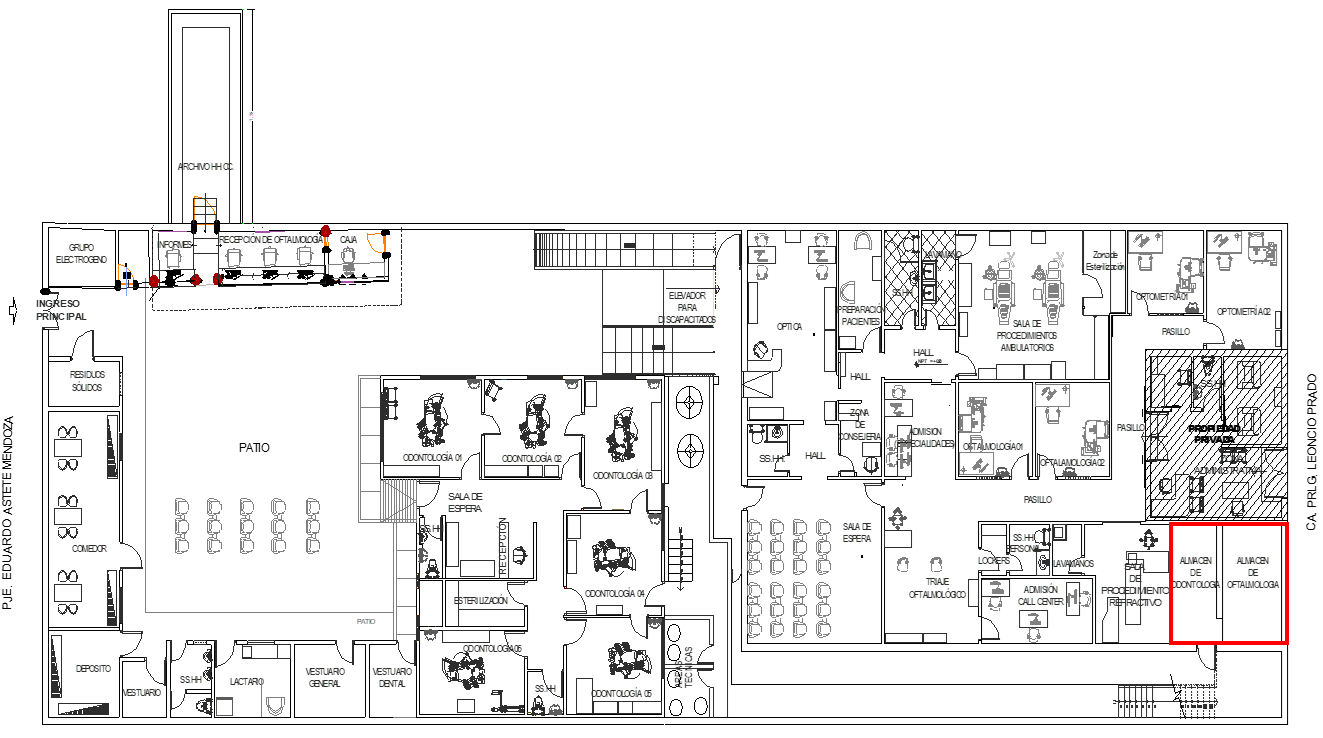
\includegraphics[width=24cm, height=14.5cm]{images/PLANO1.png}}
\end{figure}

\begin{figure}[H]
  {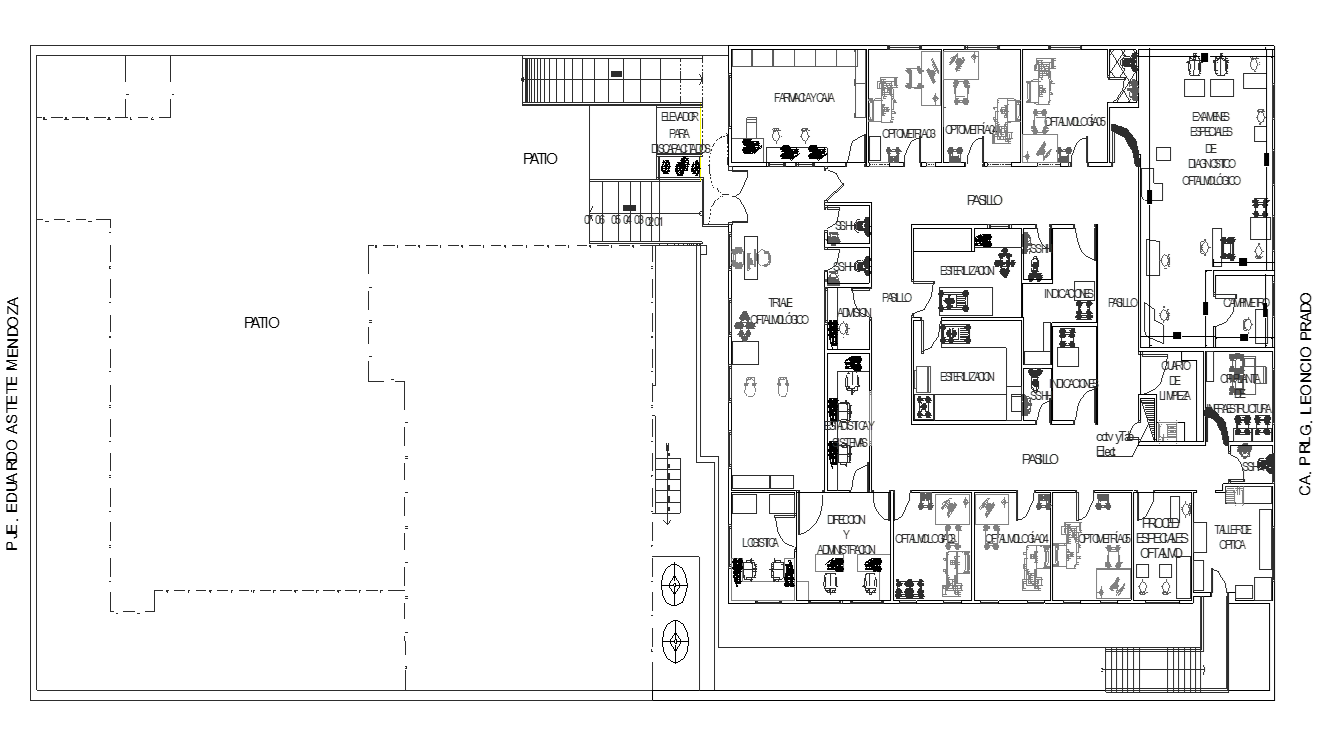
\includegraphics[width=24cm, height=15cm]{images/PLANO2.png}}
\end{figure}
\end{landscape}

\section{Solicitud de realización de la investigación}
\begin{figure}[H]
  {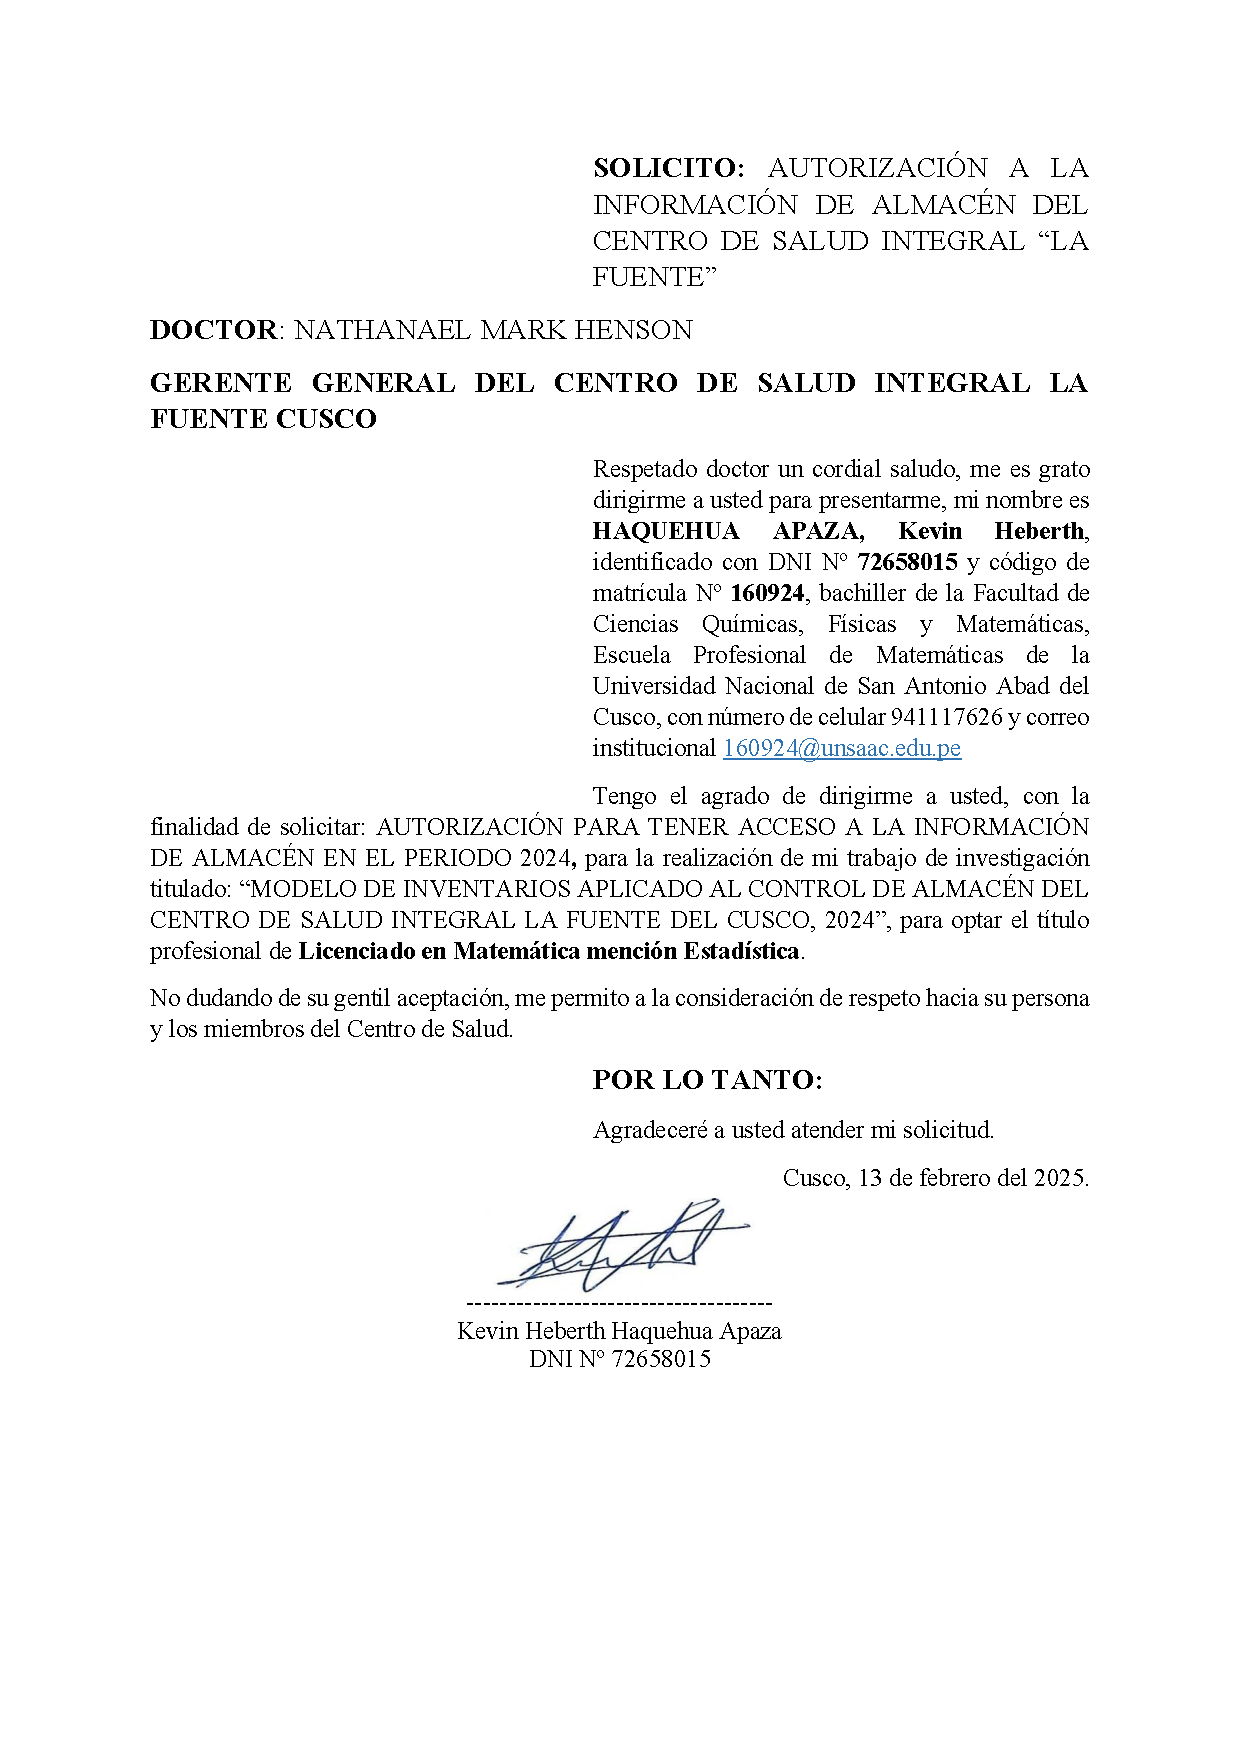
\includegraphics[width=17cm, height=23cm, trim=2cm 4cm 1.5cm 2cm, clip]{images/SOLICITUD.pdf}}
\end{figure}

\section{Autorización del Centro de Salud}
\begin{figure}[H]
  {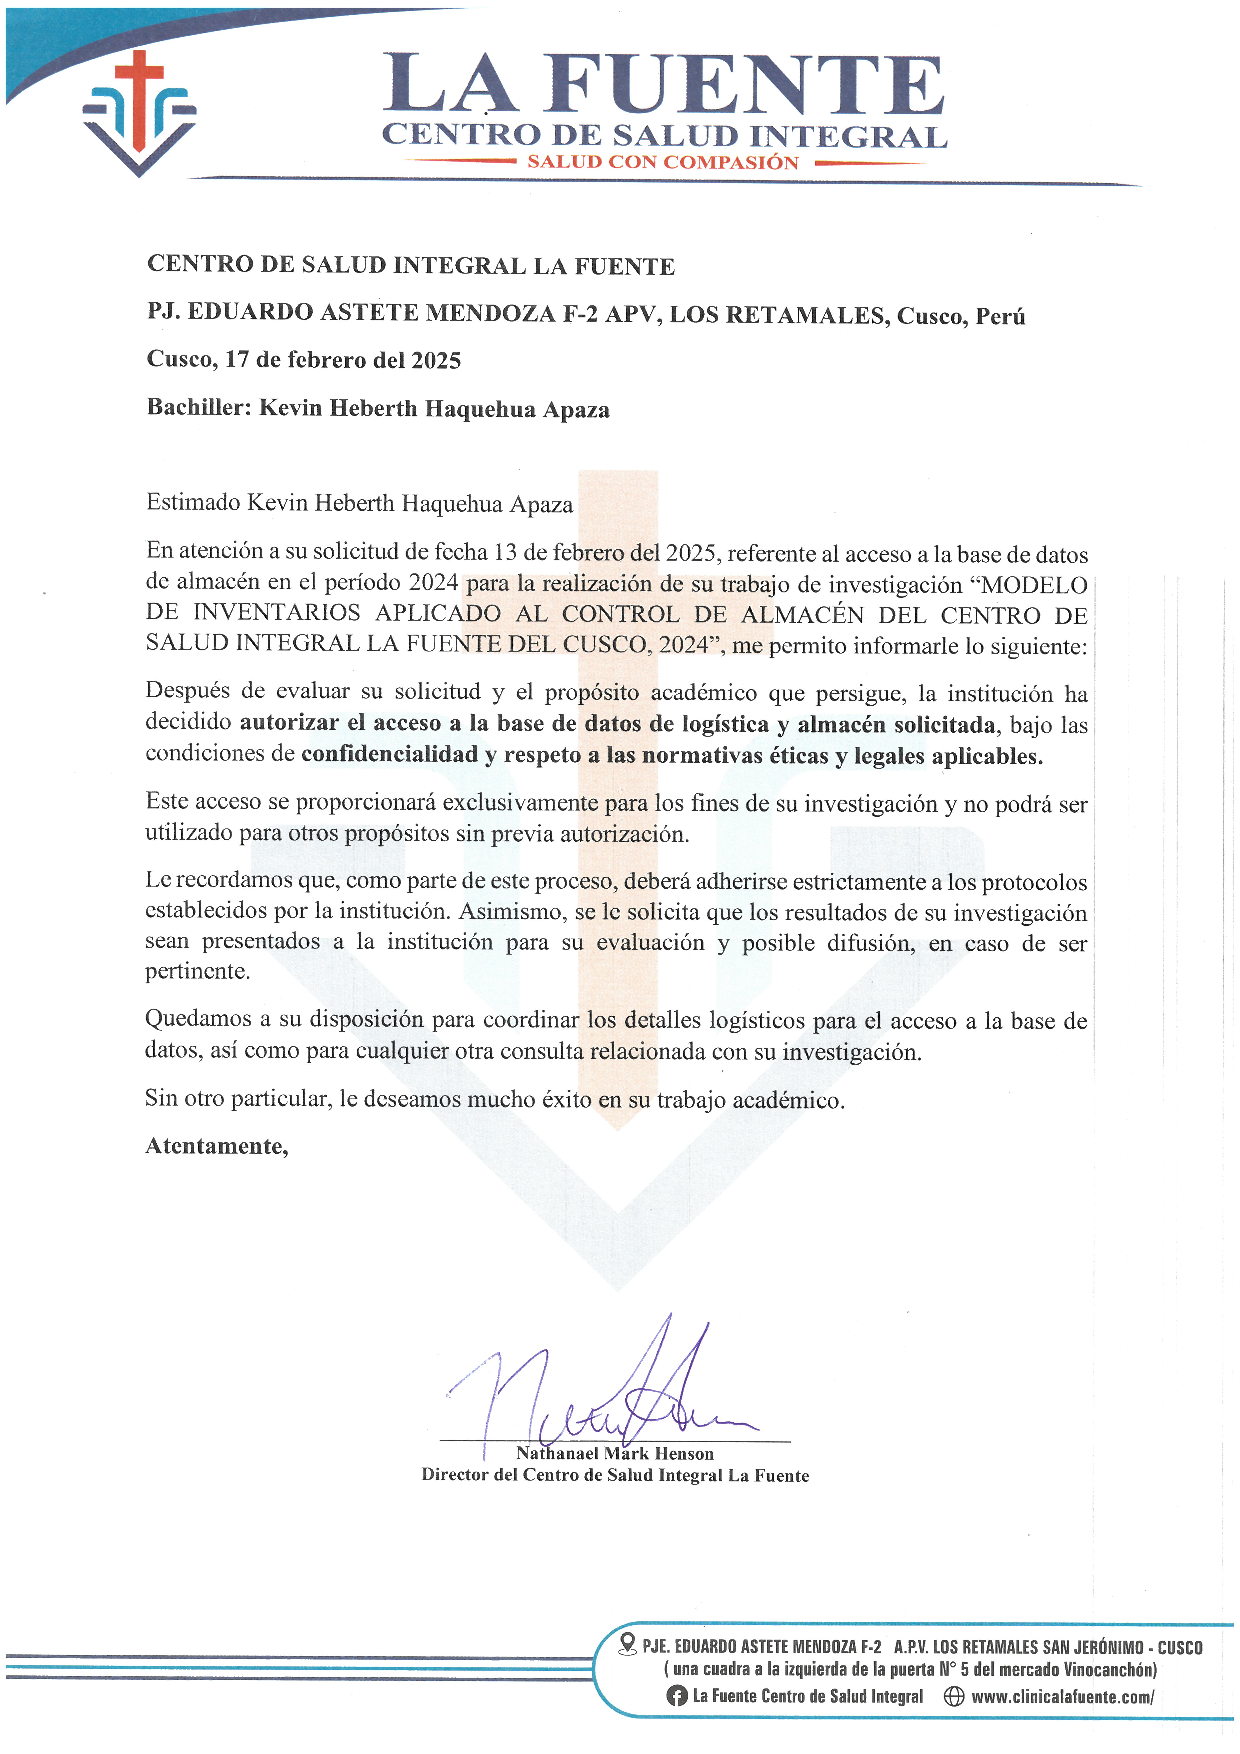
\includegraphics[width=17cm, height=23cm]{images/AUTORIZACION.pdf}}
\end{figure}

\section{Evidencia fotográfica}
\begin{figure}[H]
  {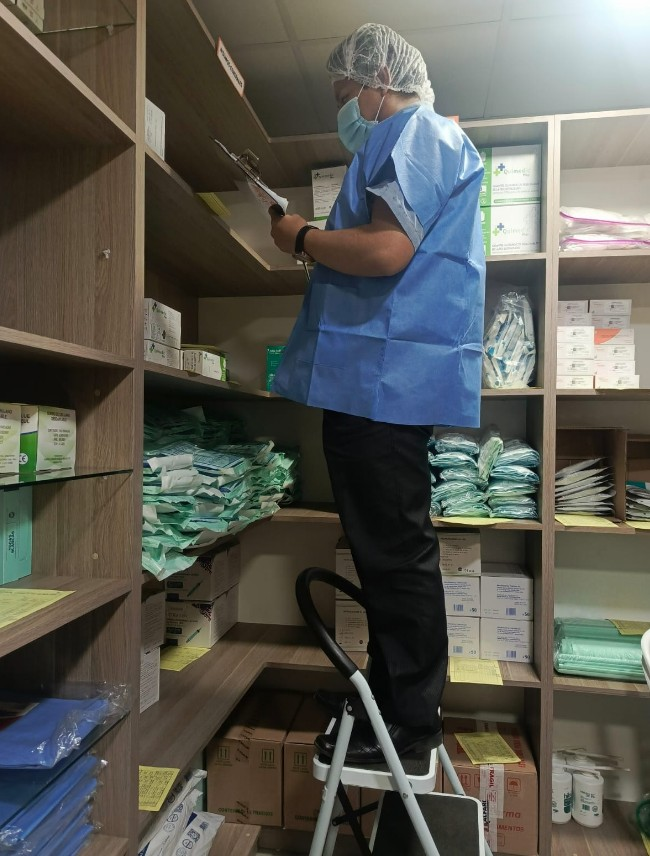
\includegraphics[width=15cm, height=11cm]{images/foto1.jpg}}
  {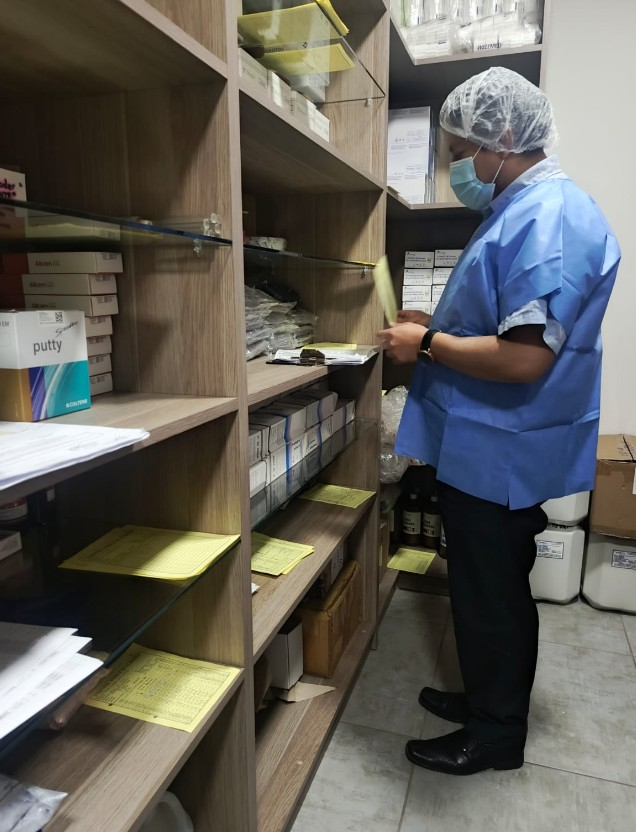
\includegraphics[width=15cm, height=11cm]{images/foto2.jpg}}
\end{figure}

\begin{figure}[H]
  {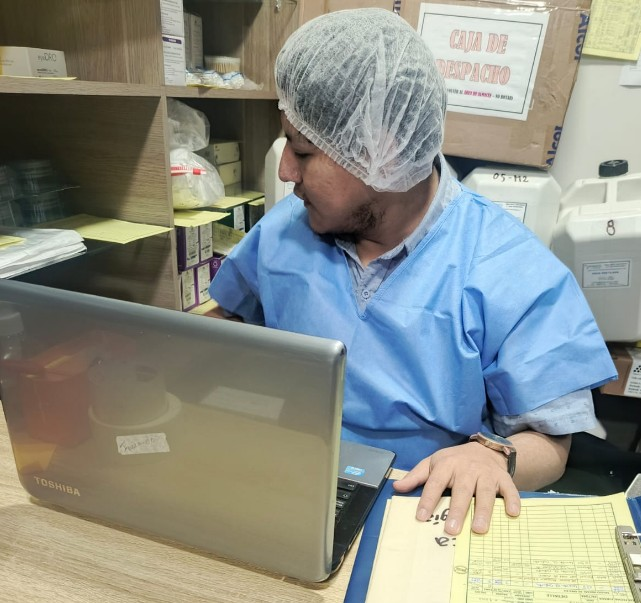
\includegraphics[width=15cm, height=11cm]{images/foto3.jpg}}
  {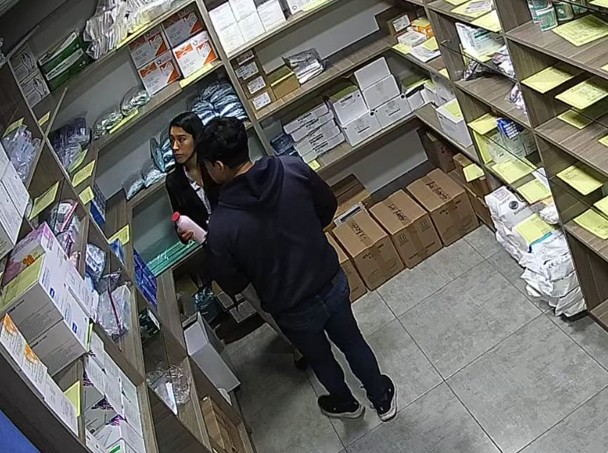
\includegraphics[width=15cm, height=11cm]{images/foto4.jpg}}
\end{figure}

\newpage
\section{Script código R}
\begin{figure}[h!]
        \begin{tcolorbox}[colback=white, colframe=black, boxrule=1.5pt, sharp corners=all]
            {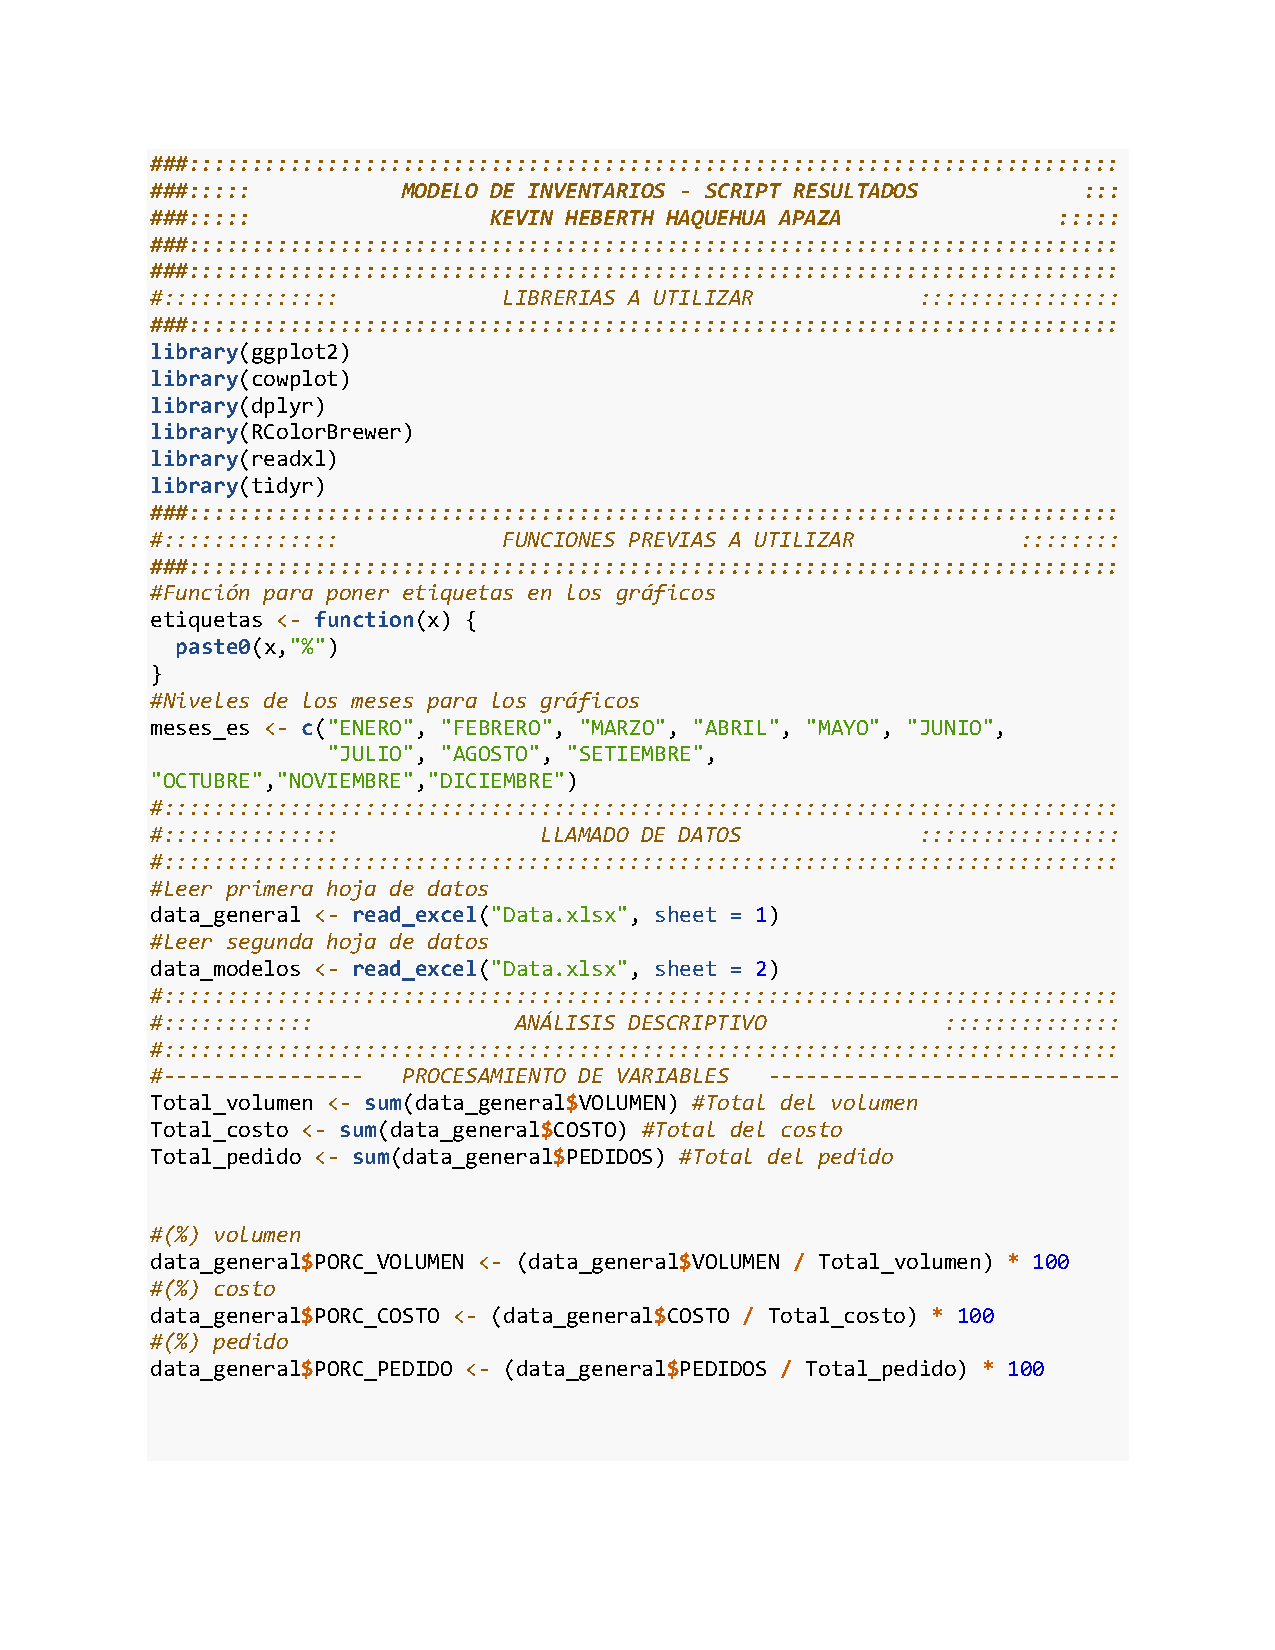
\includegraphics[width=\linewidth, height=22cm, trim=2.5cm 2.75cm 2.5cm 2.5cm, clip]{images/script1.pdf}}
        \end{tcolorbox}
\end{figure}

\begin{figure}[h!]
        \begin{tcolorbox}[colback=white, colframe=black, boxrule=1.5pt, sharp corners=all]
            {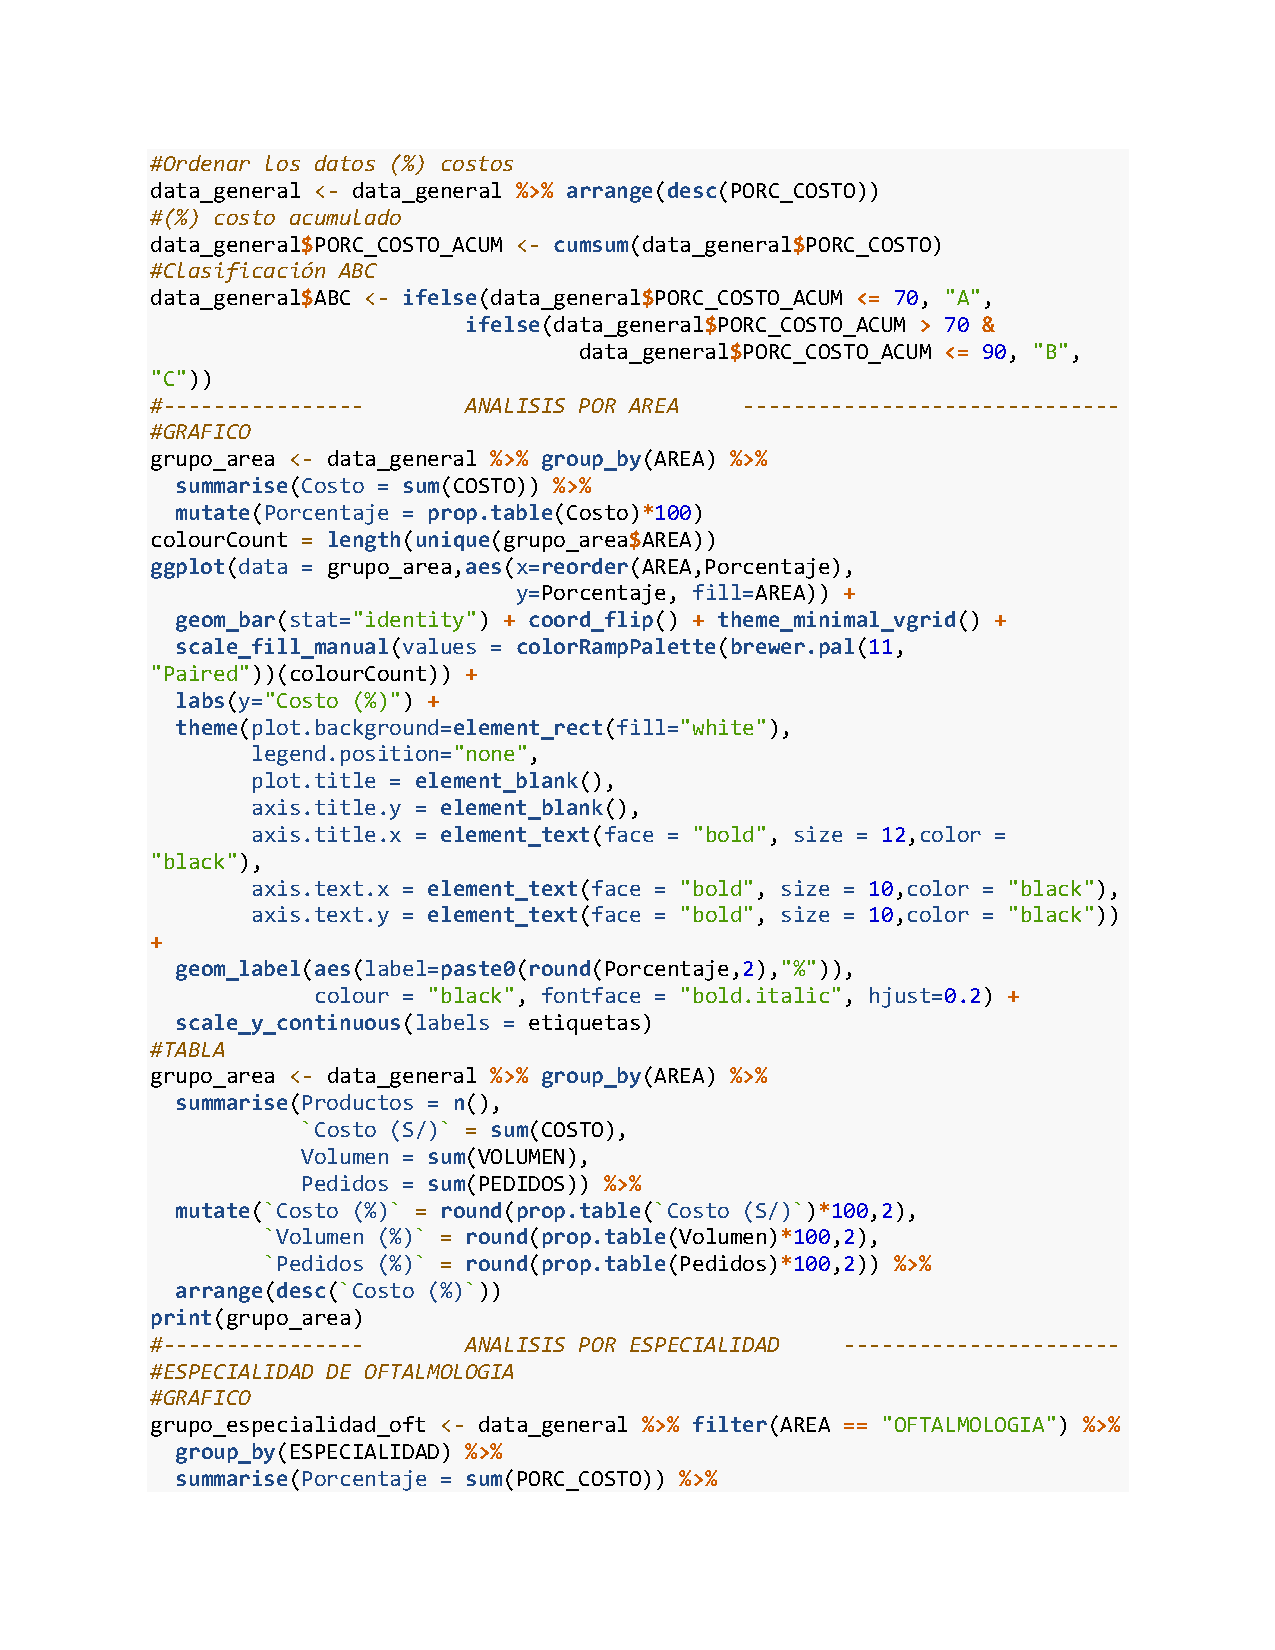
\includegraphics[width=\linewidth, height=22cm, trim=2.5cm 2.75cm 2.5cm 2.5cm, clip]{images/script2.pdf}}
        \end{tcolorbox}
\end{figure}

\begin{figure}[h!]
        \begin{tcolorbox}[colback=white, colframe=black, boxrule=1.5pt, sharp corners=all]
            {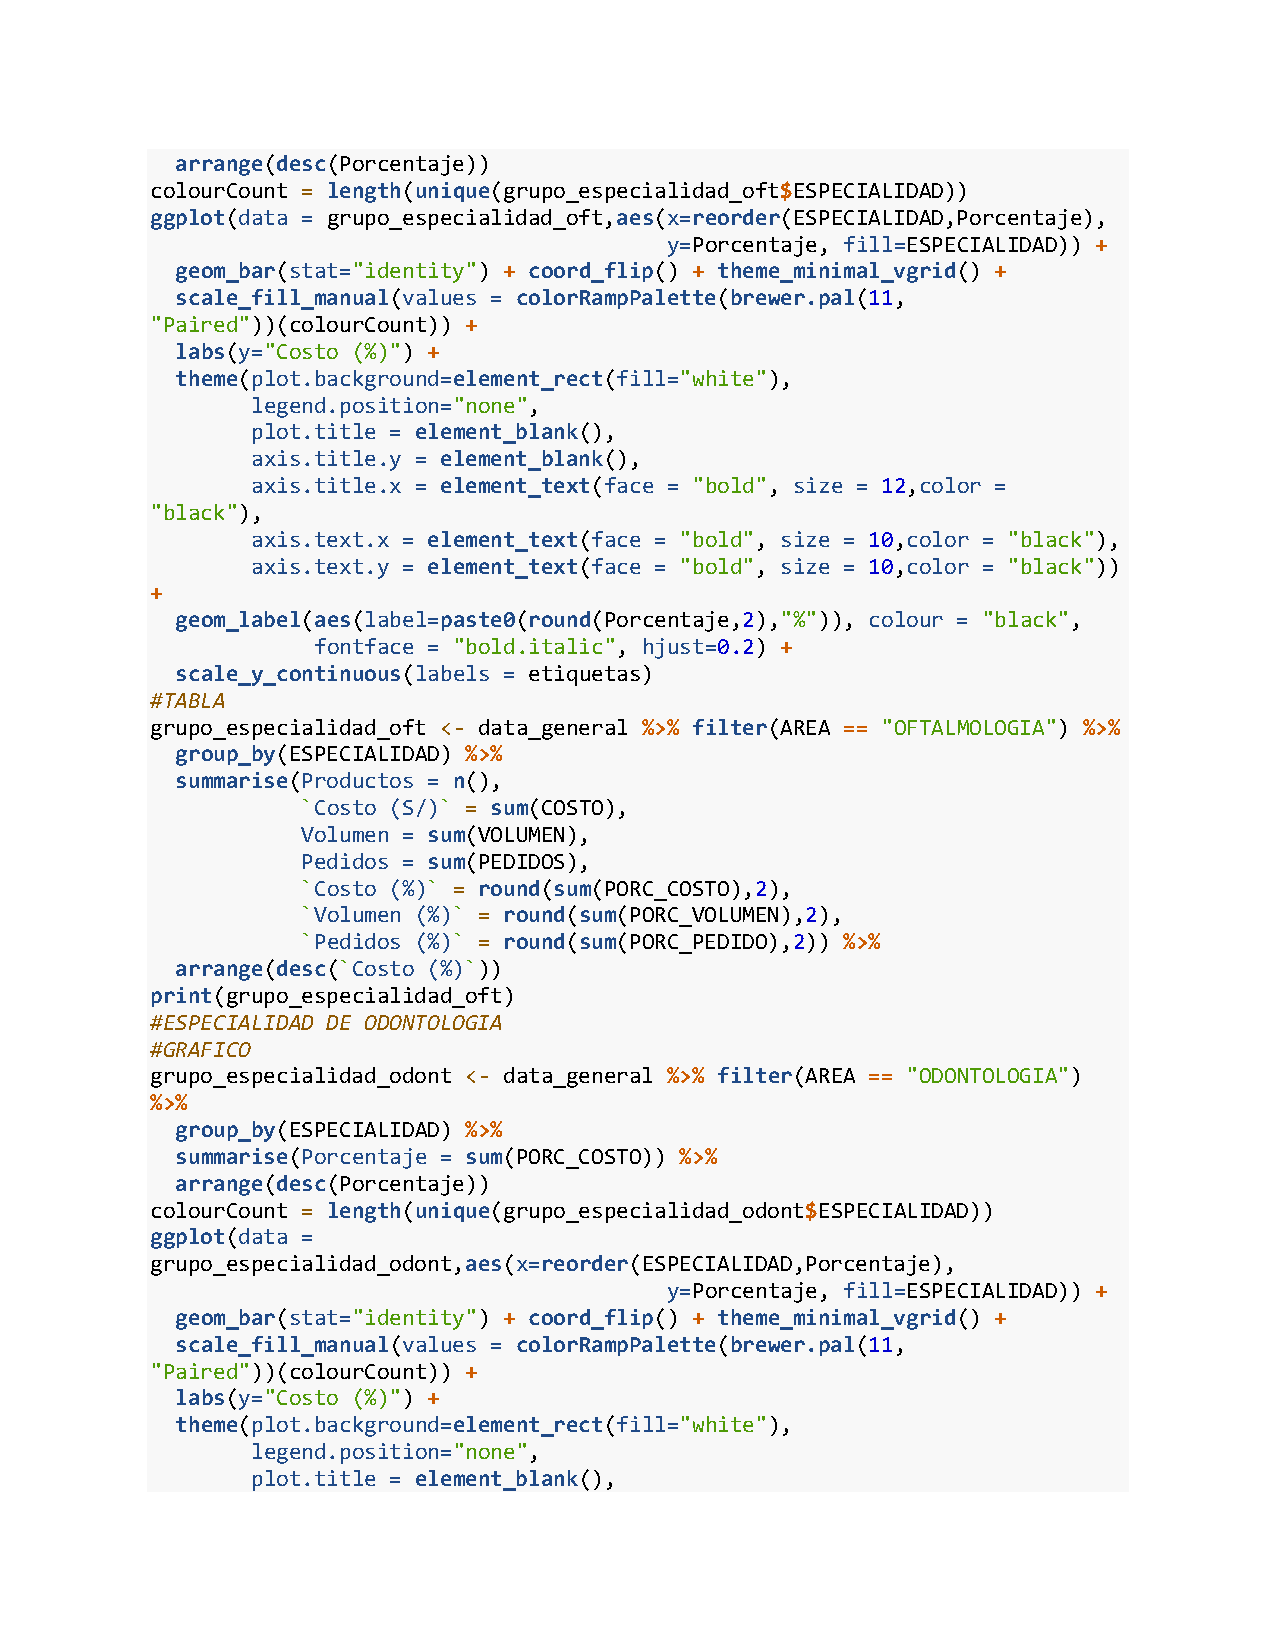
\includegraphics[width=\linewidth, height=22cm, trim=2.5cm 2.75cm 2.5cm 2.5cm, clip]{images/script3.pdf}}
        \end{tcolorbox}
\end{figure}

\begin{figure}[h!]
        \begin{tcolorbox}[colback=white, colframe=black, boxrule=1.5pt, sharp corners=all]
            {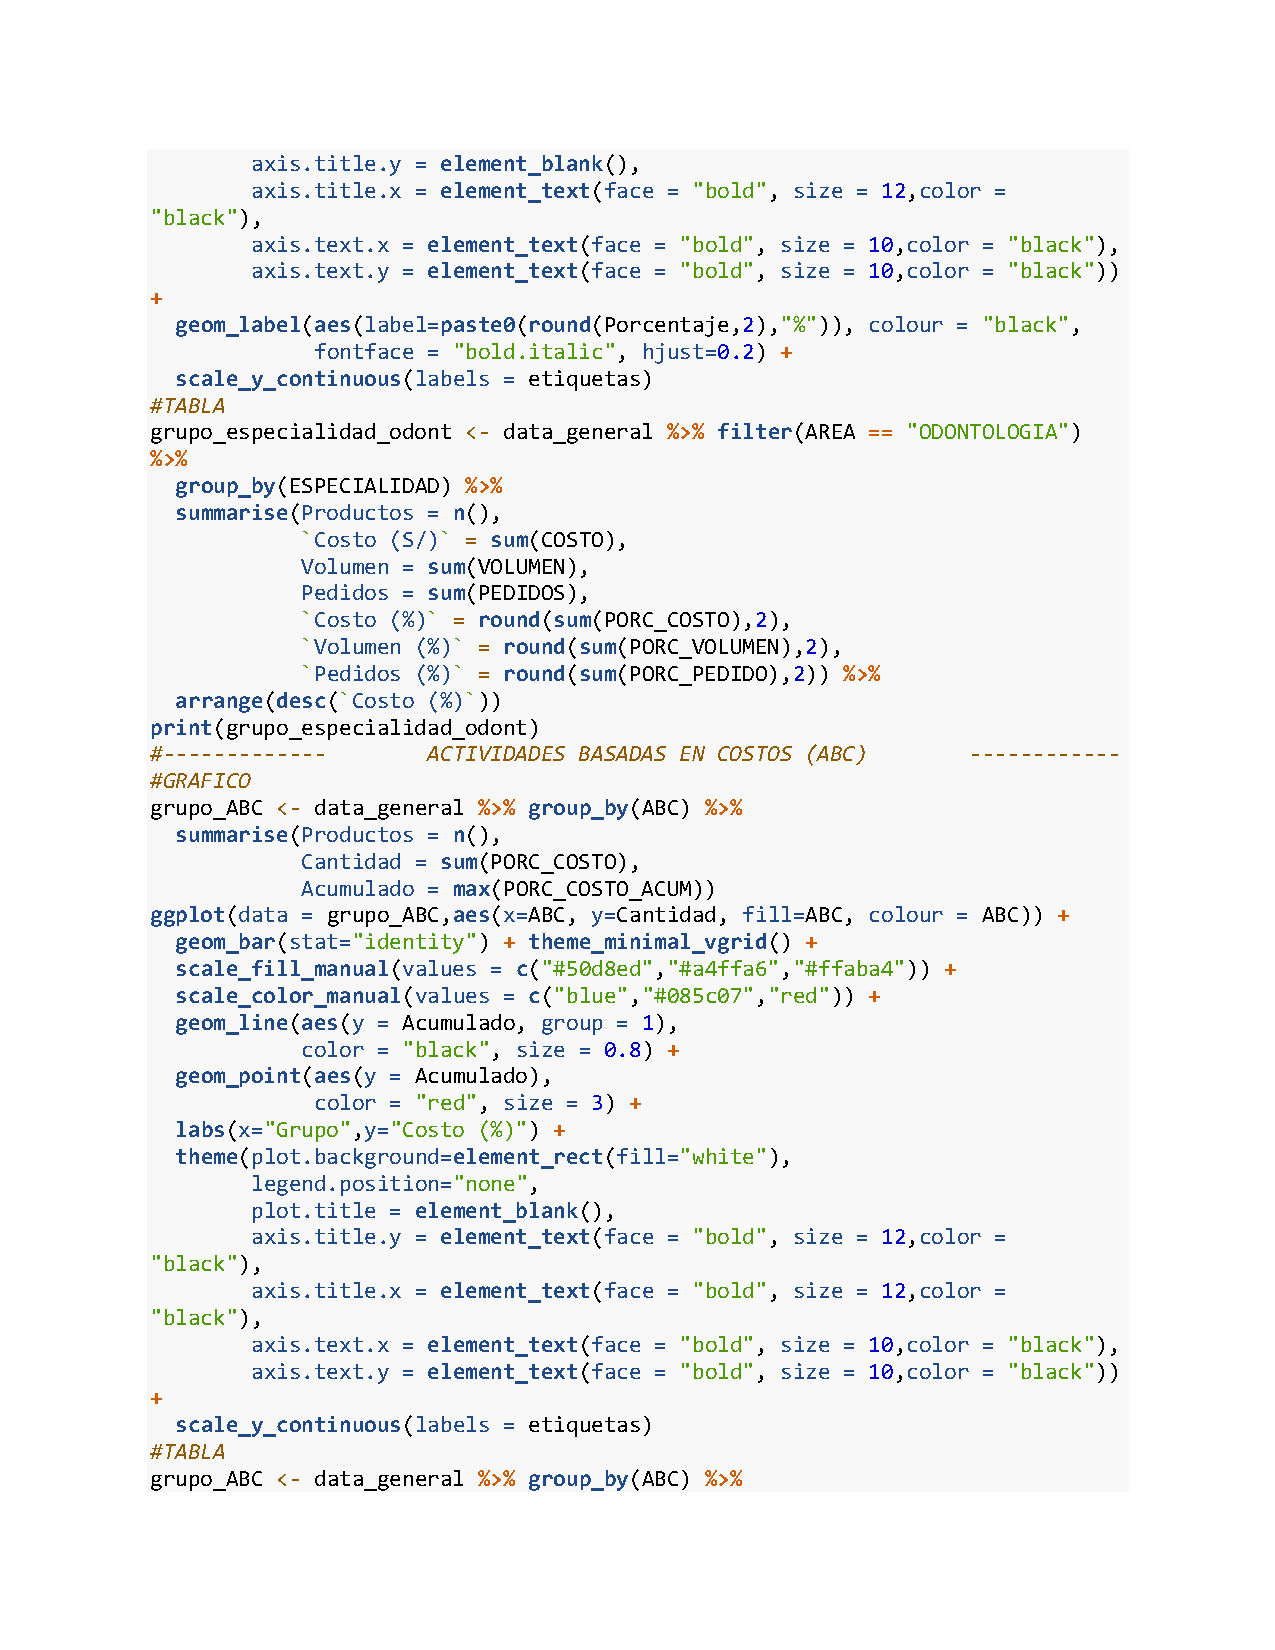
\includegraphics[width=\linewidth, height=22cm, trim=2.5cm 2.75cm 2.5cm 2.5cm, clip]{images/script4.pdf}}
        \end{tcolorbox}
\end{figure}

\begin{figure}[h!]
        \begin{tcolorbox}[colback=white, colframe=black, boxrule=1.5pt, sharp corners=all]
            {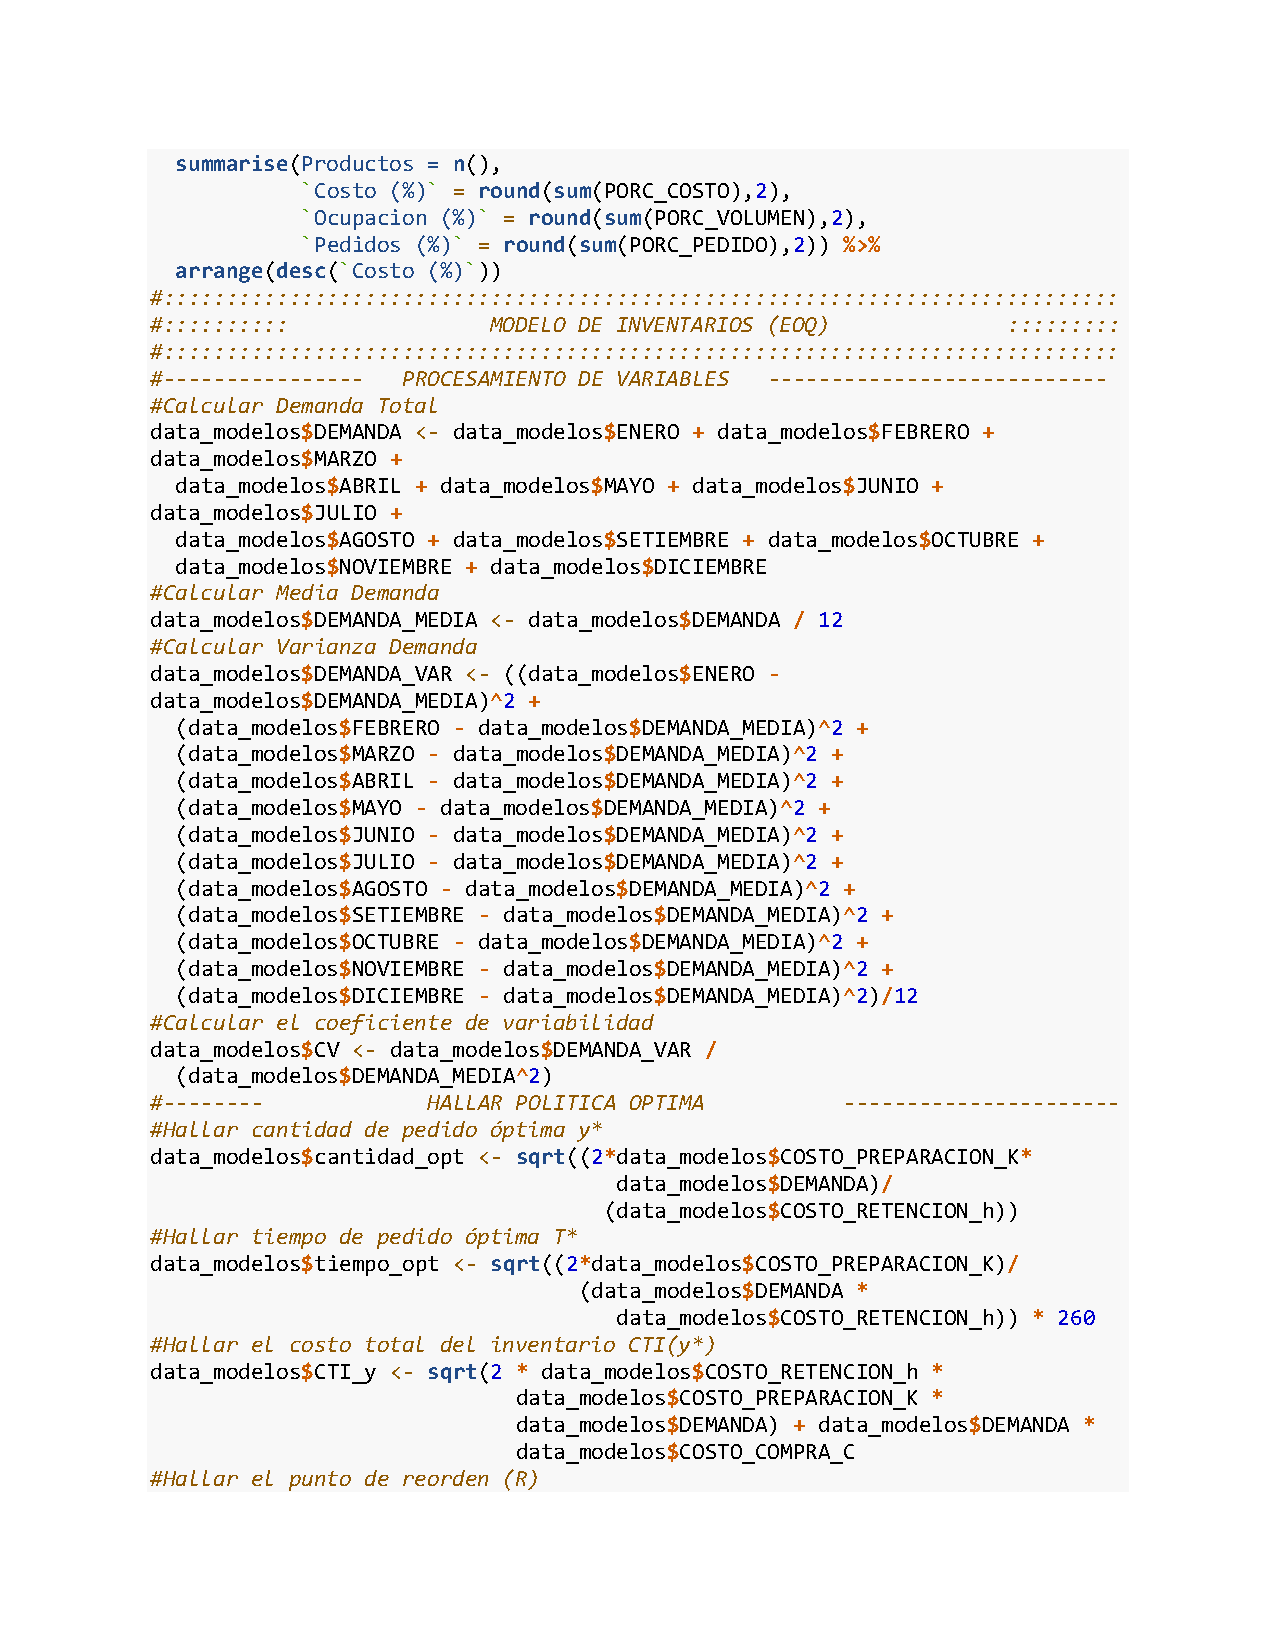
\includegraphics[width=\linewidth, height=22cm, trim=2.5cm 2.75cm 2.5cm 2.5cm, clip]{images/script5.pdf}}
        \end{tcolorbox}
\end{figure}

\begin{figure}[h!]
        \begin{tcolorbox}[colback=white, colframe=black, boxrule=1.5pt, sharp corners=all]
            {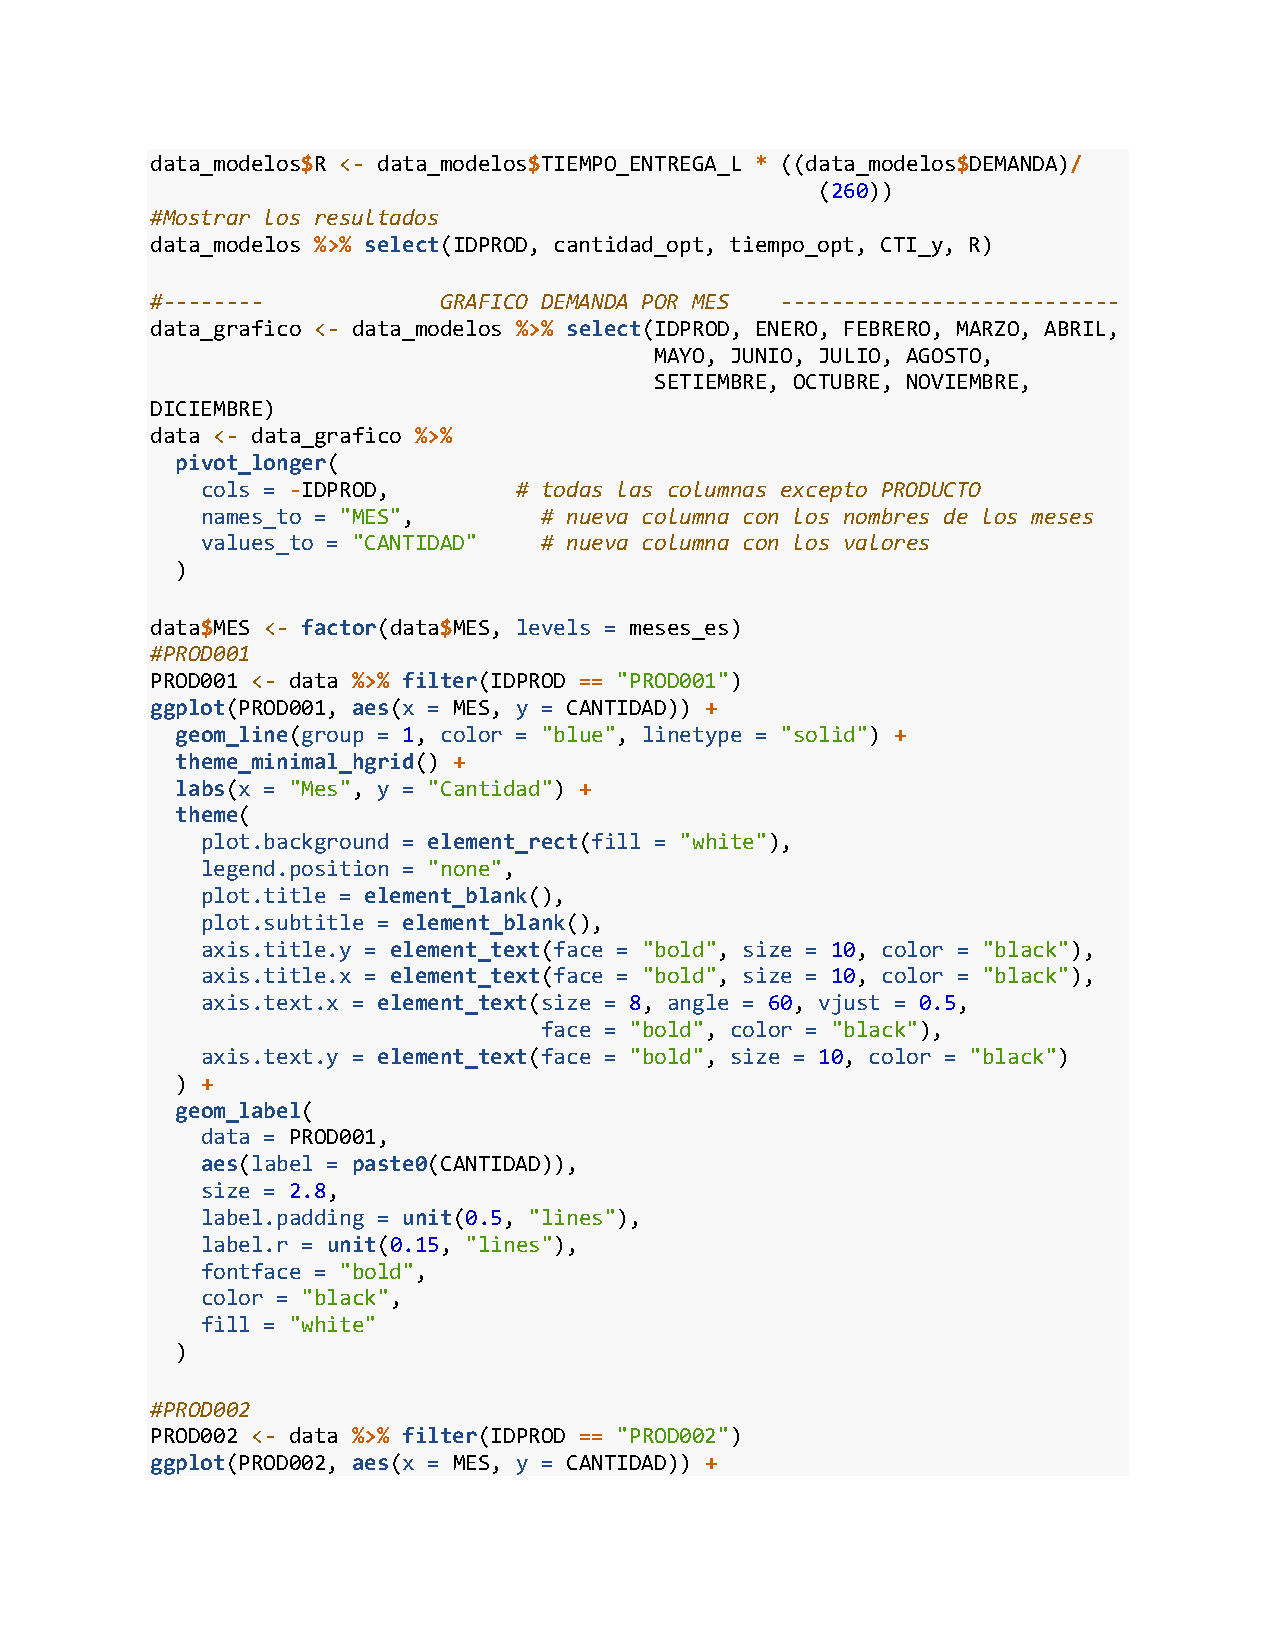
\includegraphics[width=\linewidth, height=22cm, trim=2.5cm 2.75cm 2.5cm 2.5cm, clip]{images/script6.pdf}}
        \end{tcolorbox}
\end{figure}

\begin{figure}[h!]
        \begin{tcolorbox}[colback=white, colframe=black, boxrule=1.5pt, sharp corners=all]
            {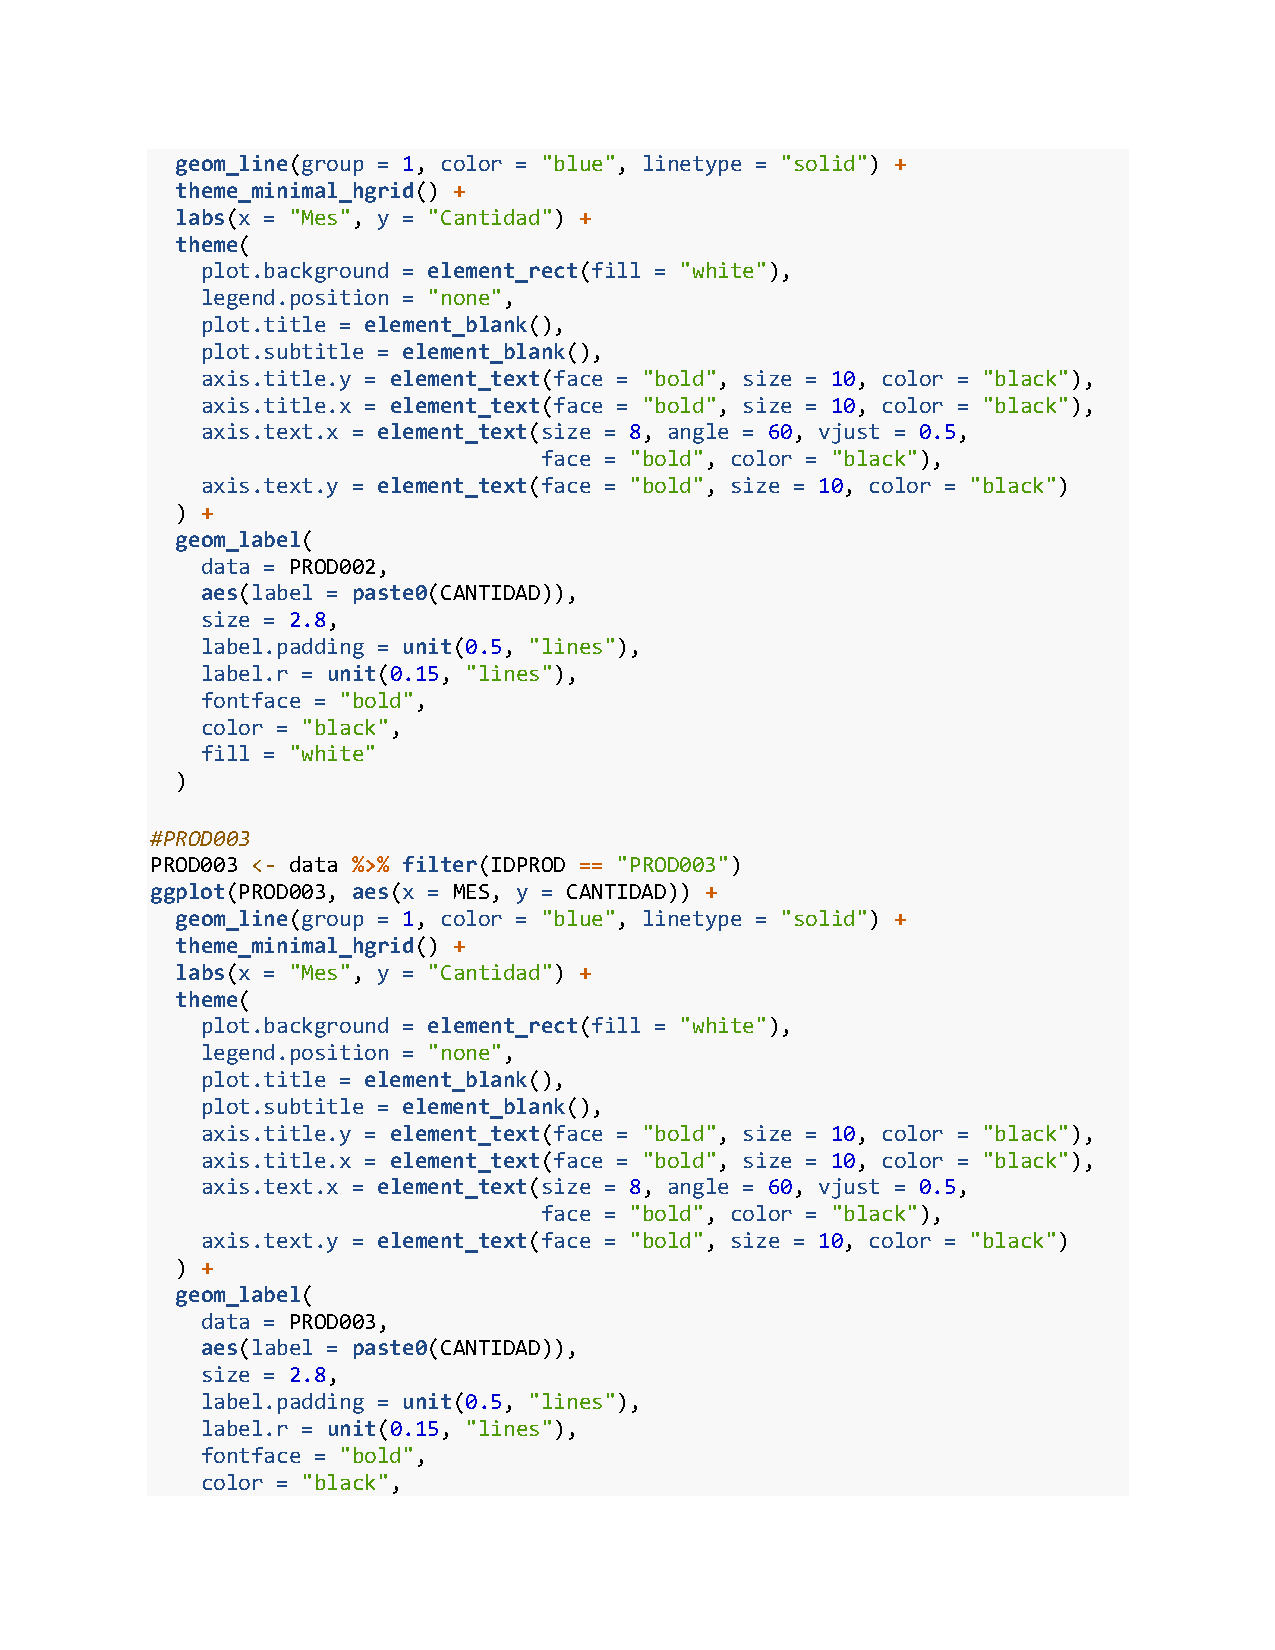
\includegraphics[width=\linewidth, height=22cm, trim=2.5cm 2.5cm 2.5cm 2.5cm, clip]{images/script7.pdf}}
        \end{tcolorbox}
\end{figure}

\begin{figure}[h!]
        \begin{tcolorbox}[colback=white, colframe=black, boxrule=1.5pt, sharp corners=all]
            {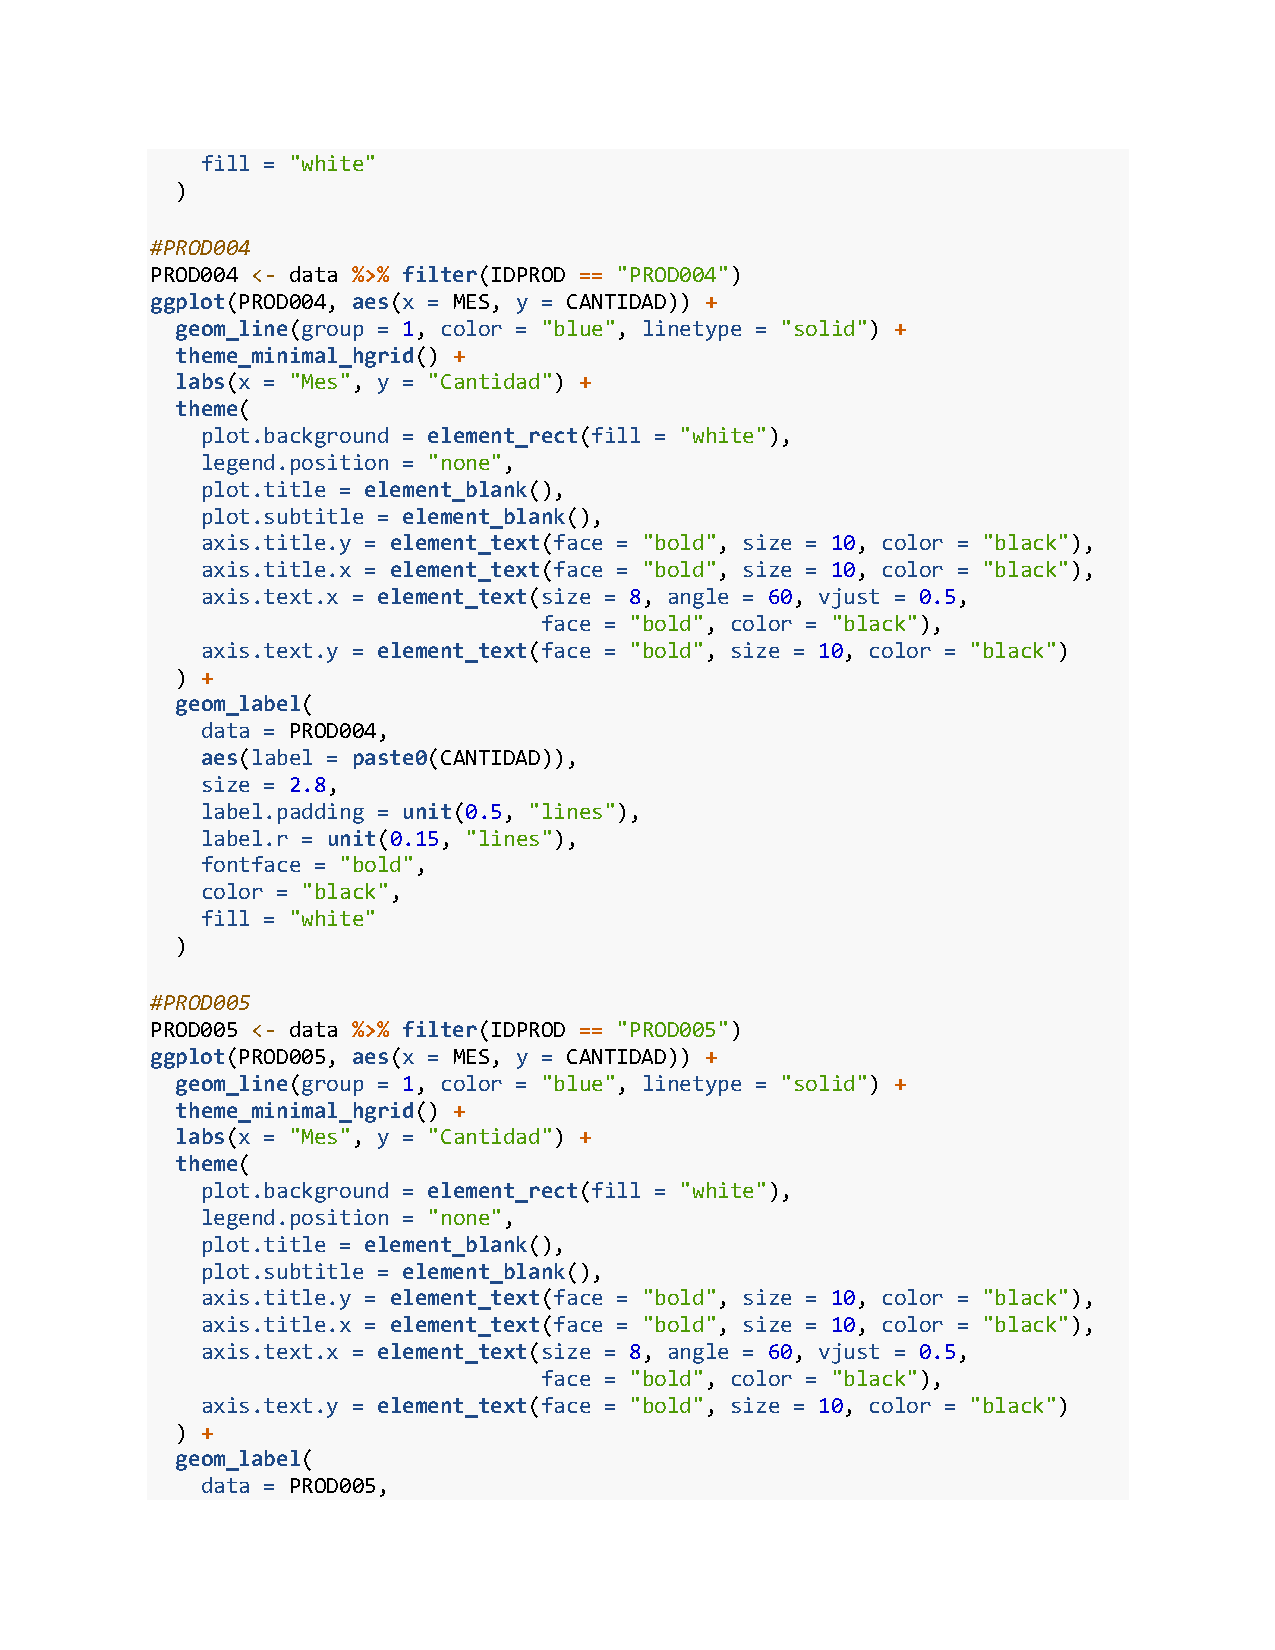
\includegraphics[width=\linewidth, height=22cm, trim=2.5cm 2.5cm 2.5cm 2.5cm, clip]{images/script8.pdf}}
        \end{tcolorbox}
\end{figure}

\begin{figure}[h!]
        \begin{tcolorbox}[colback=white, colframe=black, boxrule=1.5pt, sharp corners=all]
            {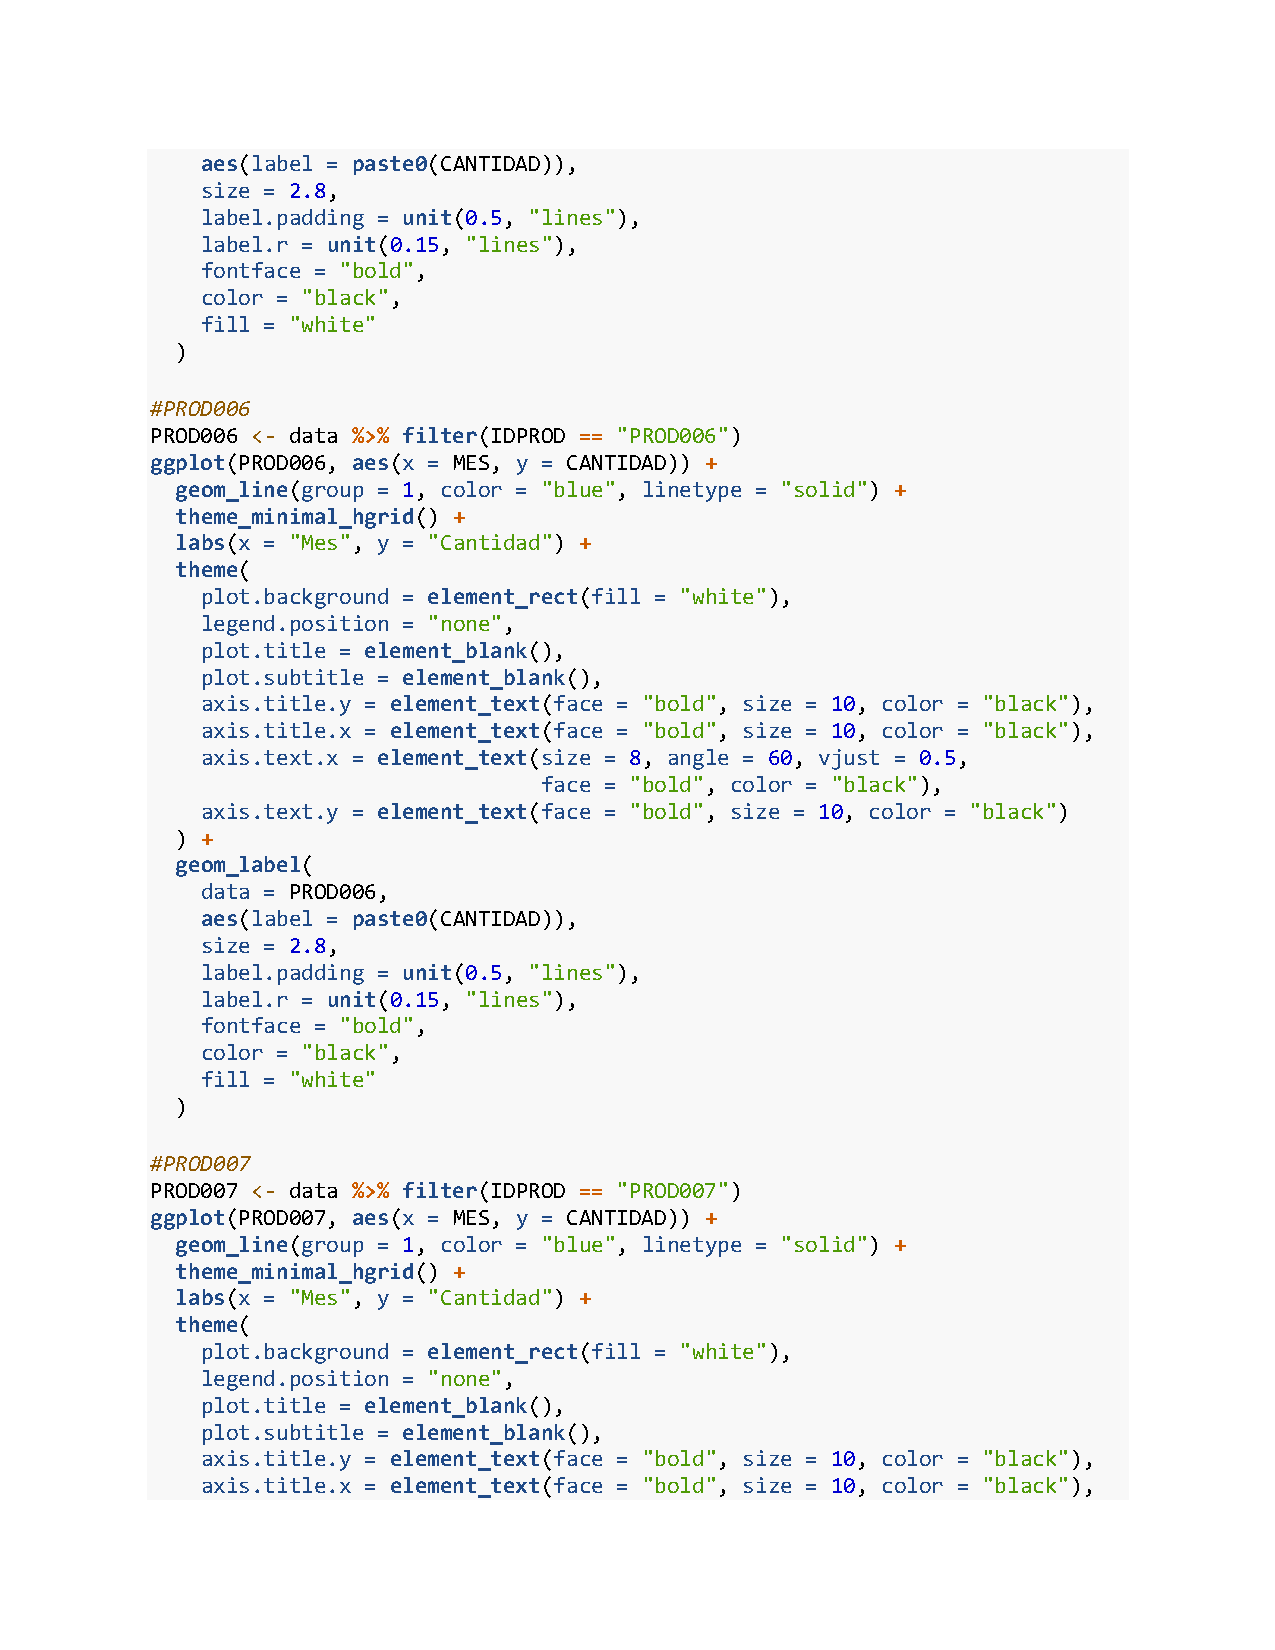
\includegraphics[width=\linewidth, height=22cm, trim=2.5cm 2.5cm 2.5cm 2.5cm, clip]{images/script9.pdf}}
        \end{tcolorbox}
\end{figure}

\begin{figure}[h!]
        \begin{tcolorbox}[colback=white, colframe=black, boxrule=1.5pt, sharp corners=all]
            {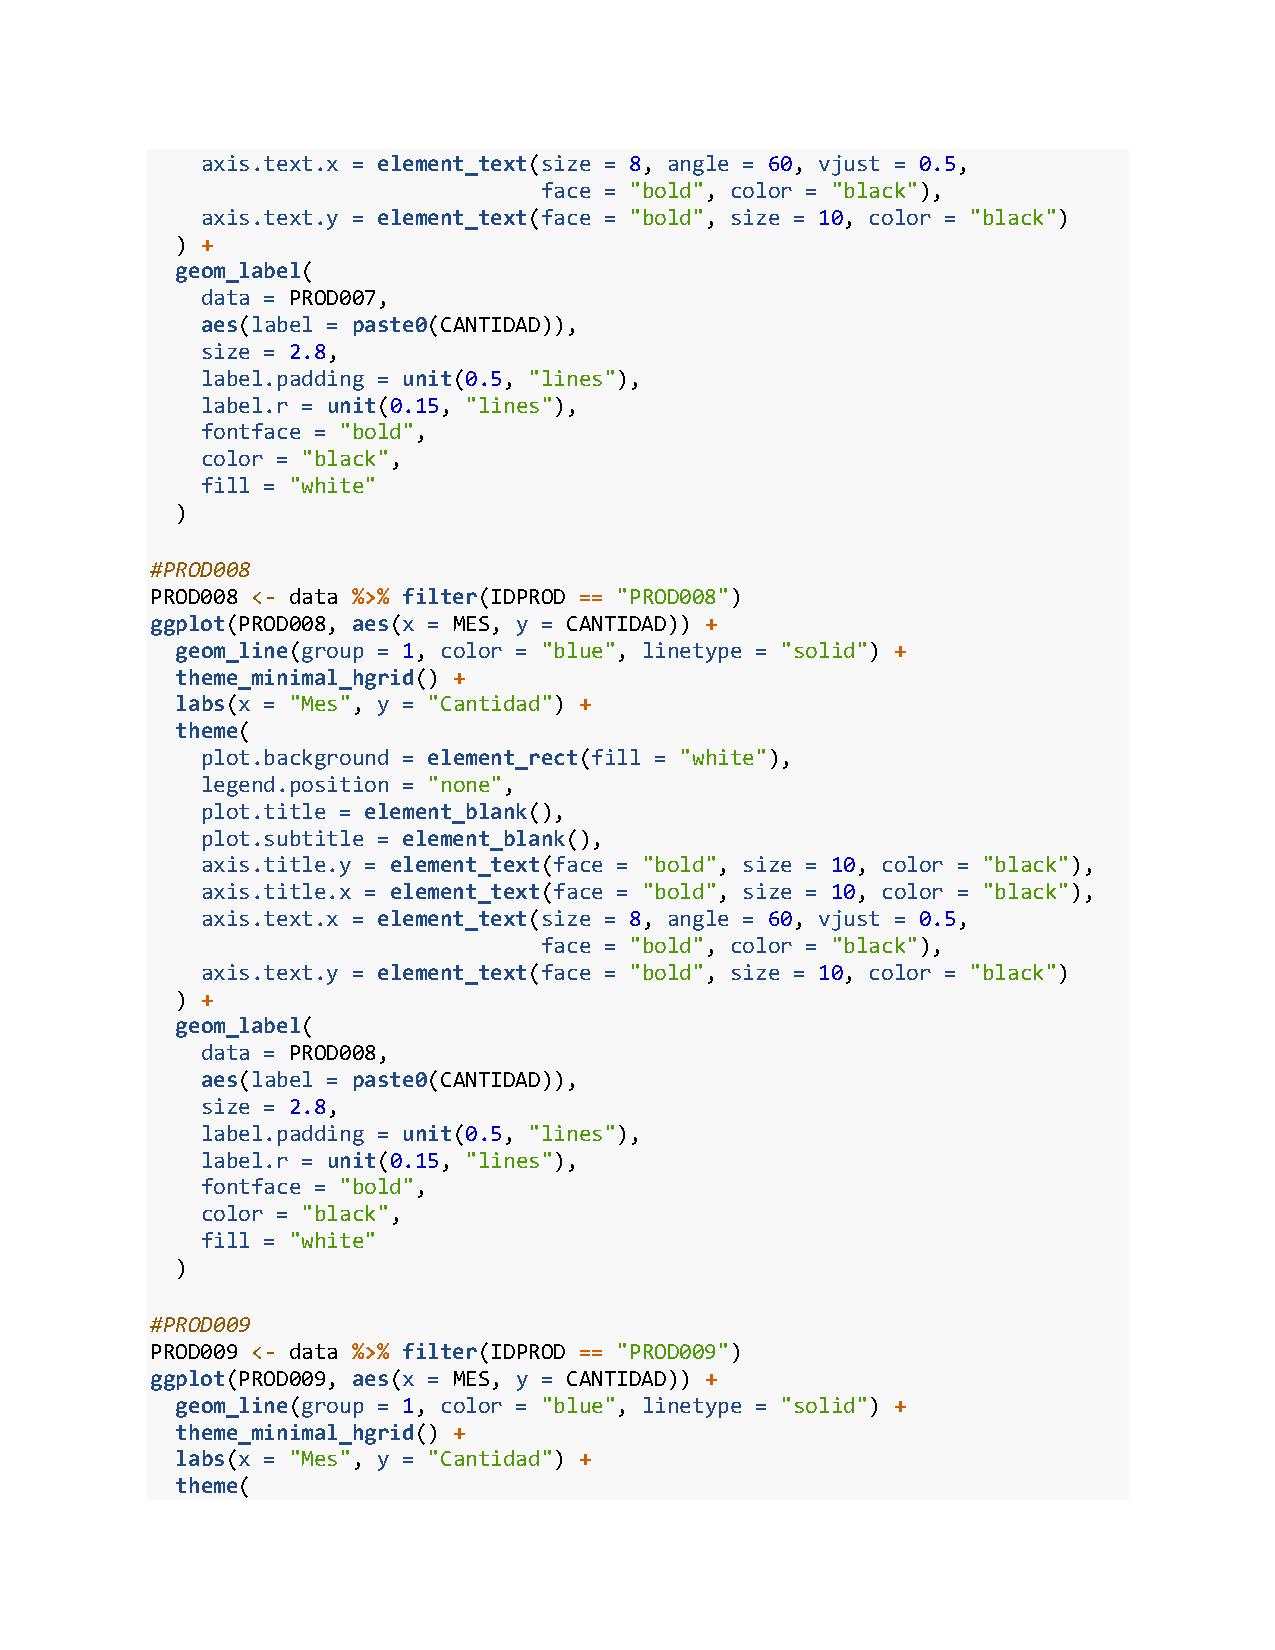
\includegraphics[width=\linewidth, height=22cm, trim=2.5cm 2.5cm 2.5cm 2.5cm, clip]{images/script10.pdf}}
        \end{tcolorbox}
\end{figure}

\begin{figure}[h!]
        \begin{tcolorbox}[colback=white, colframe=black, boxrule=1.5pt, sharp corners=all]
            {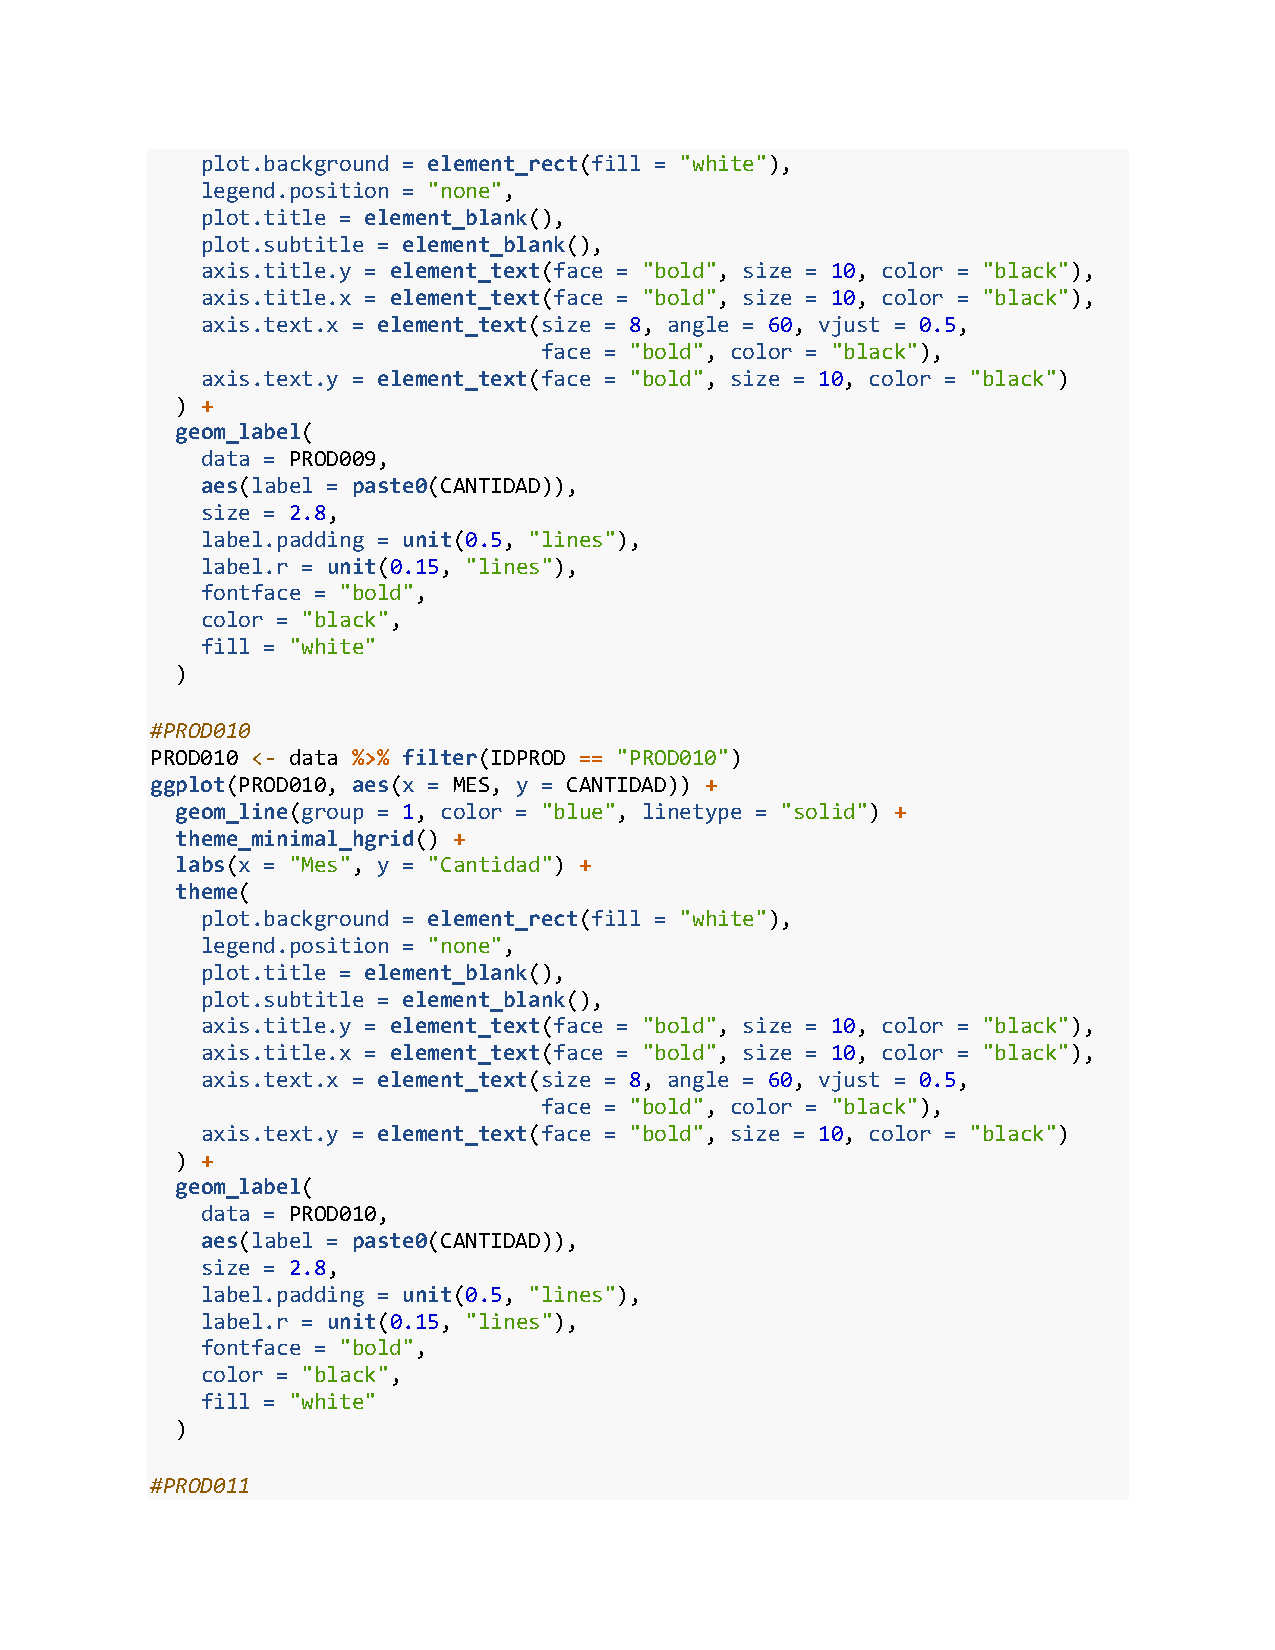
\includegraphics[width=\linewidth, height=22cm, trim=2.5cm 2.5cm 2.5cm 2.5cm, clip]{images/script11.pdf}}
        \end{tcolorbox}
\end{figure}

\begin{figure}[h!]
        \begin{tcolorbox}[colback=white, colframe=black, boxrule=1.5pt, sharp corners=all]
            {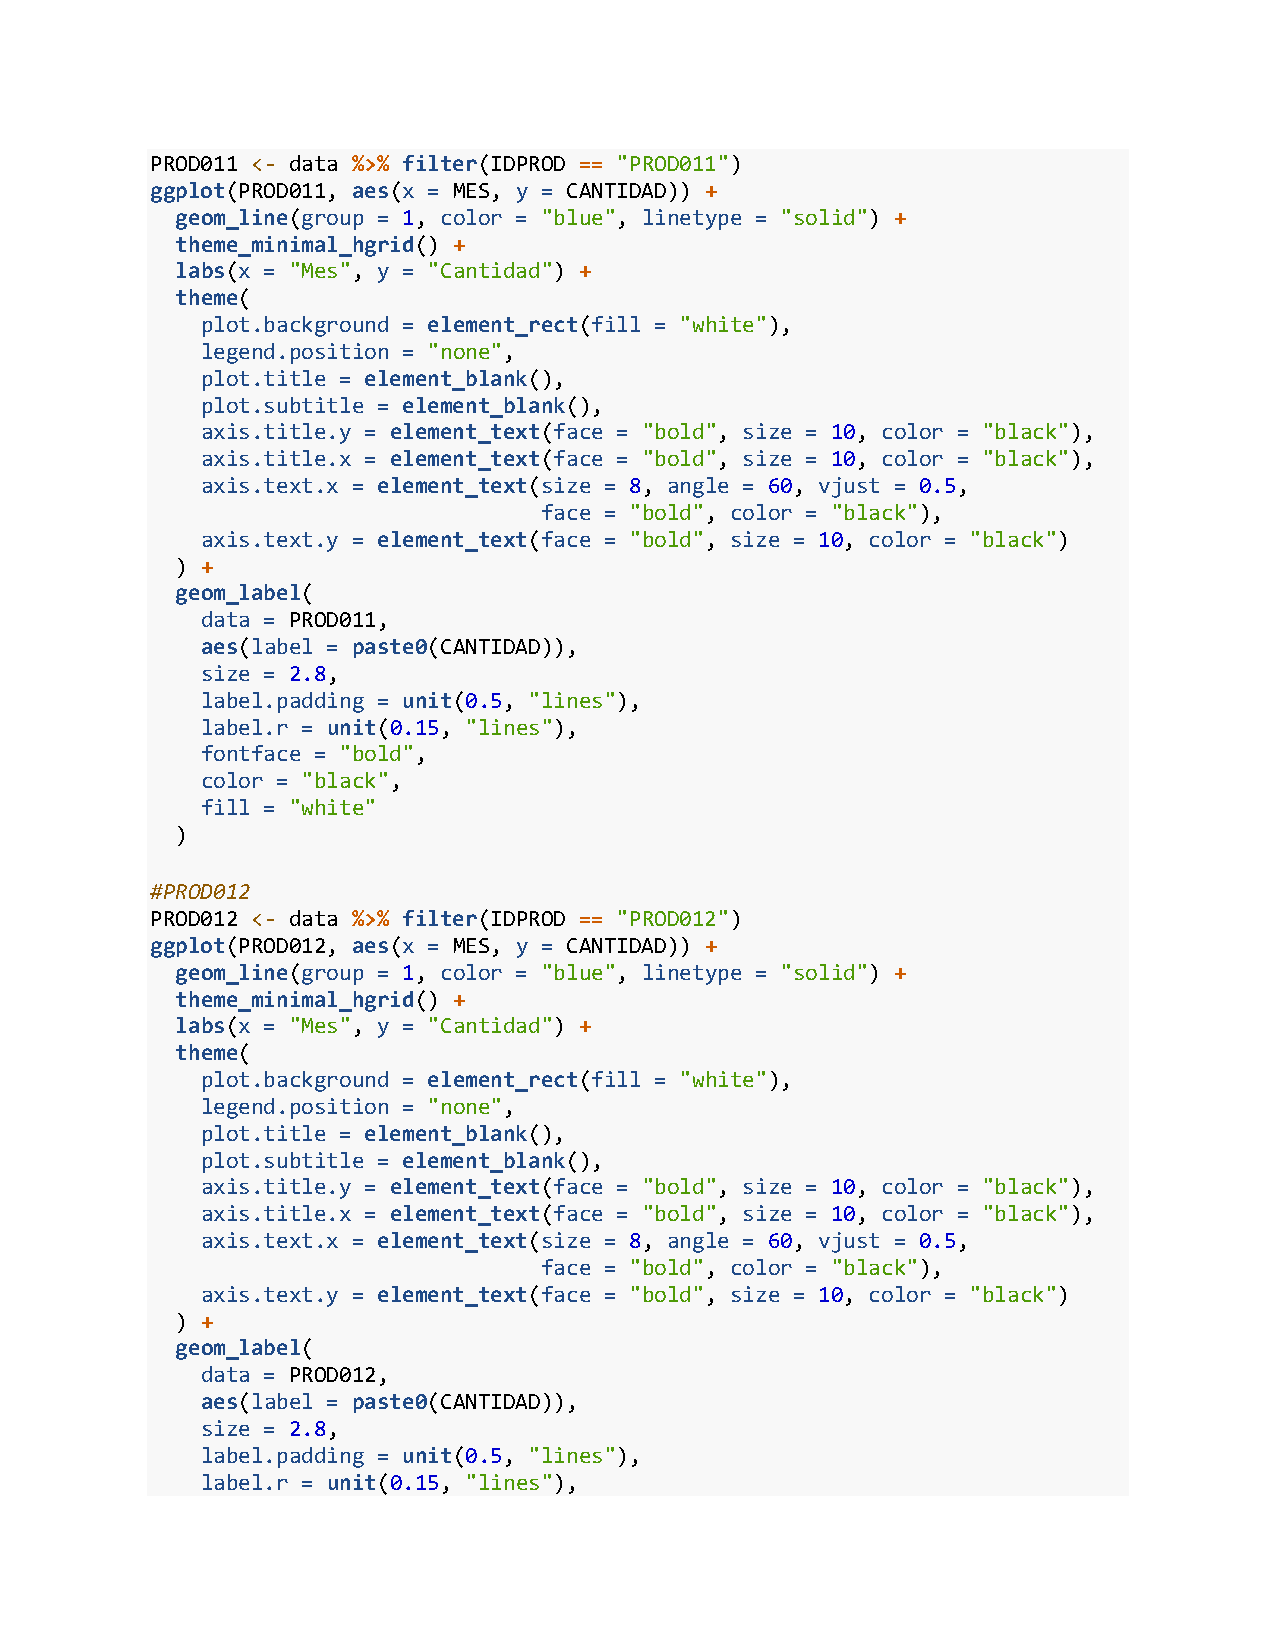
\includegraphics[width=\linewidth, height=22cm, trim=2.5cm 2.5cm 2.5cm 2.5cm, clip]{images/script12.pdf}}
        \end{tcolorbox}
\end{figure}

\begin{figure}[h!]
        \begin{tcolorbox}[colback=white, colframe=black, boxrule=1.5pt, sharp corners=all]
            {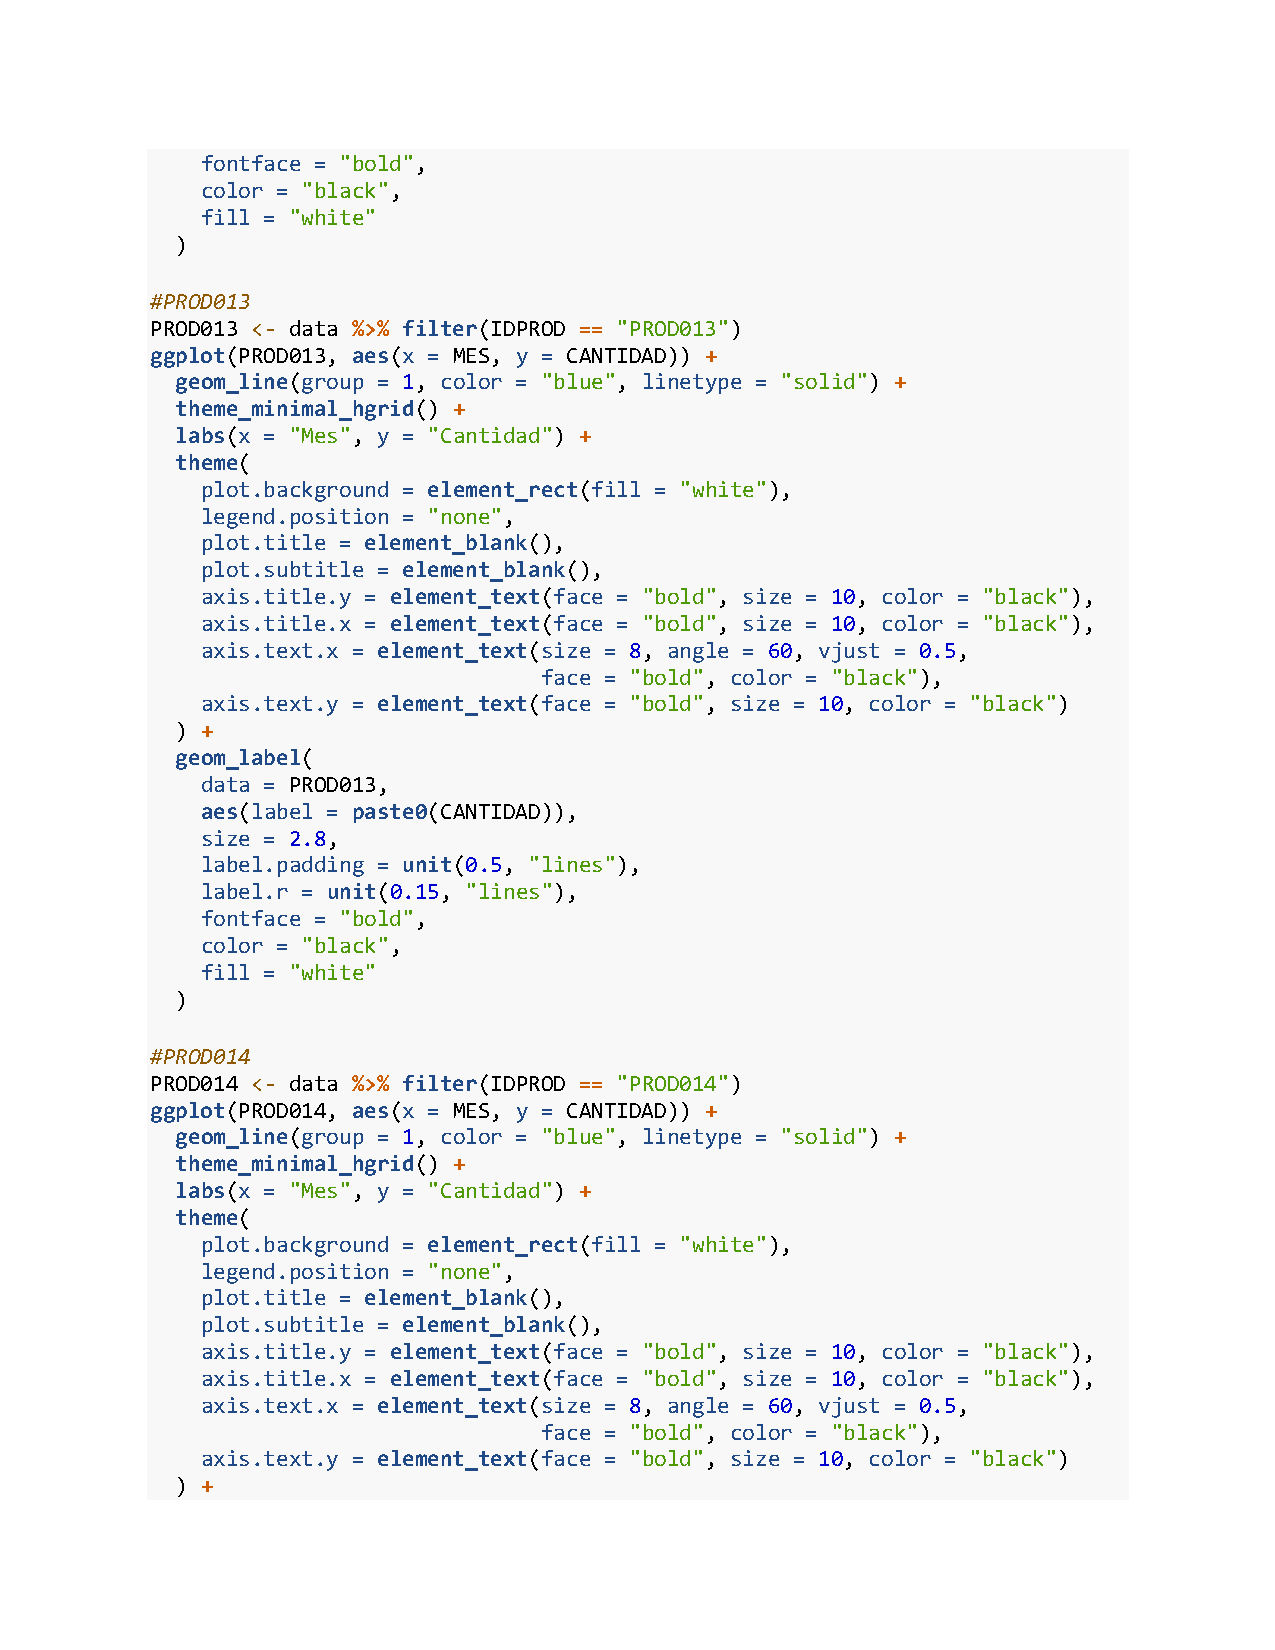
\includegraphics[width=\linewidth, height=22cm, trim=2.5cm 2.5cm 2.5cm 2.5cm, clip]{images/script13.pdf}}
        \end{tcolorbox}
\end{figure}

\begin{figure}[h!]
        \begin{tcolorbox}[colback=white, colframe=black, boxrule=1.5pt, sharp corners=all]
            {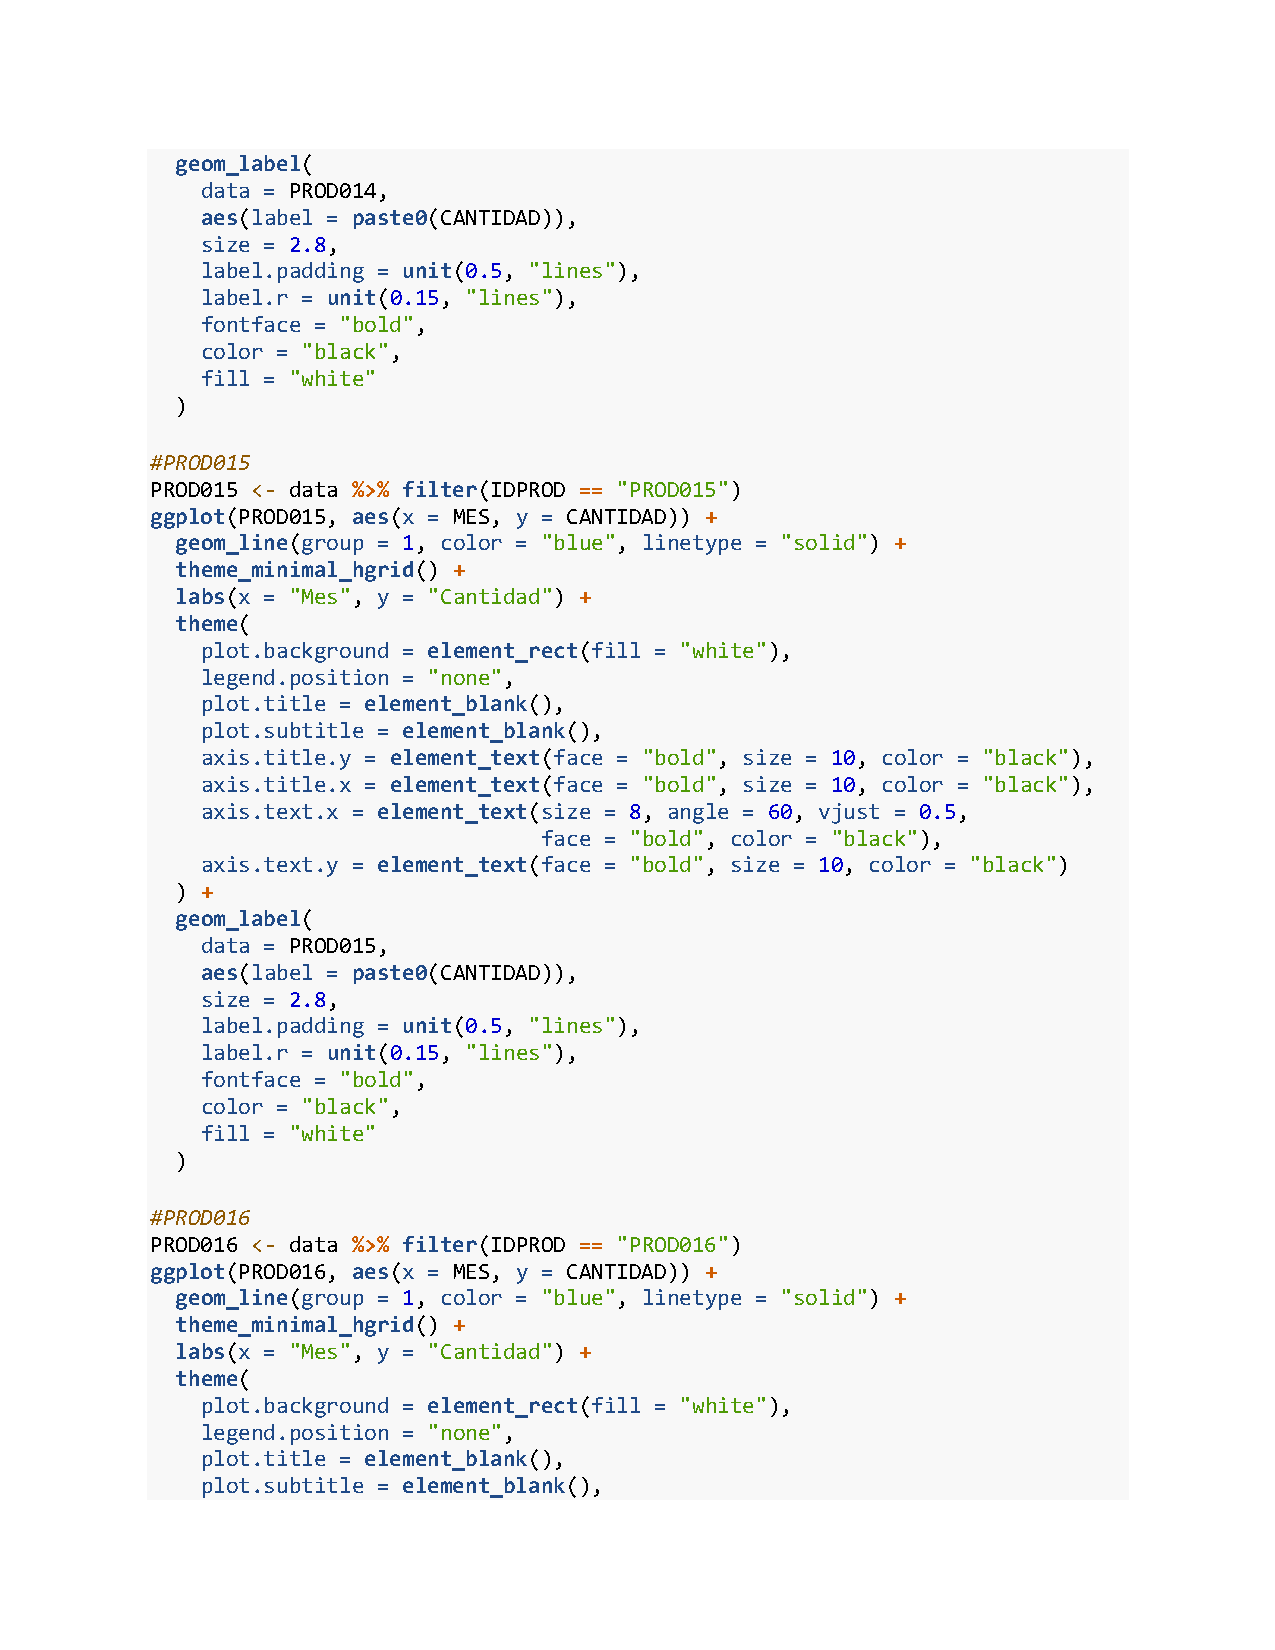
\includegraphics[width=\linewidth, height=22cm, trim=2.5cm 2.5cm 2.5cm 2.5cm, clip]{images/script14.pdf}}
        \end{tcolorbox}
\end{figure}

\begin{figure}[h!]
        \begin{tcolorbox}[colback=white, colframe=black, boxrule=1.5pt, sharp corners=all]
            {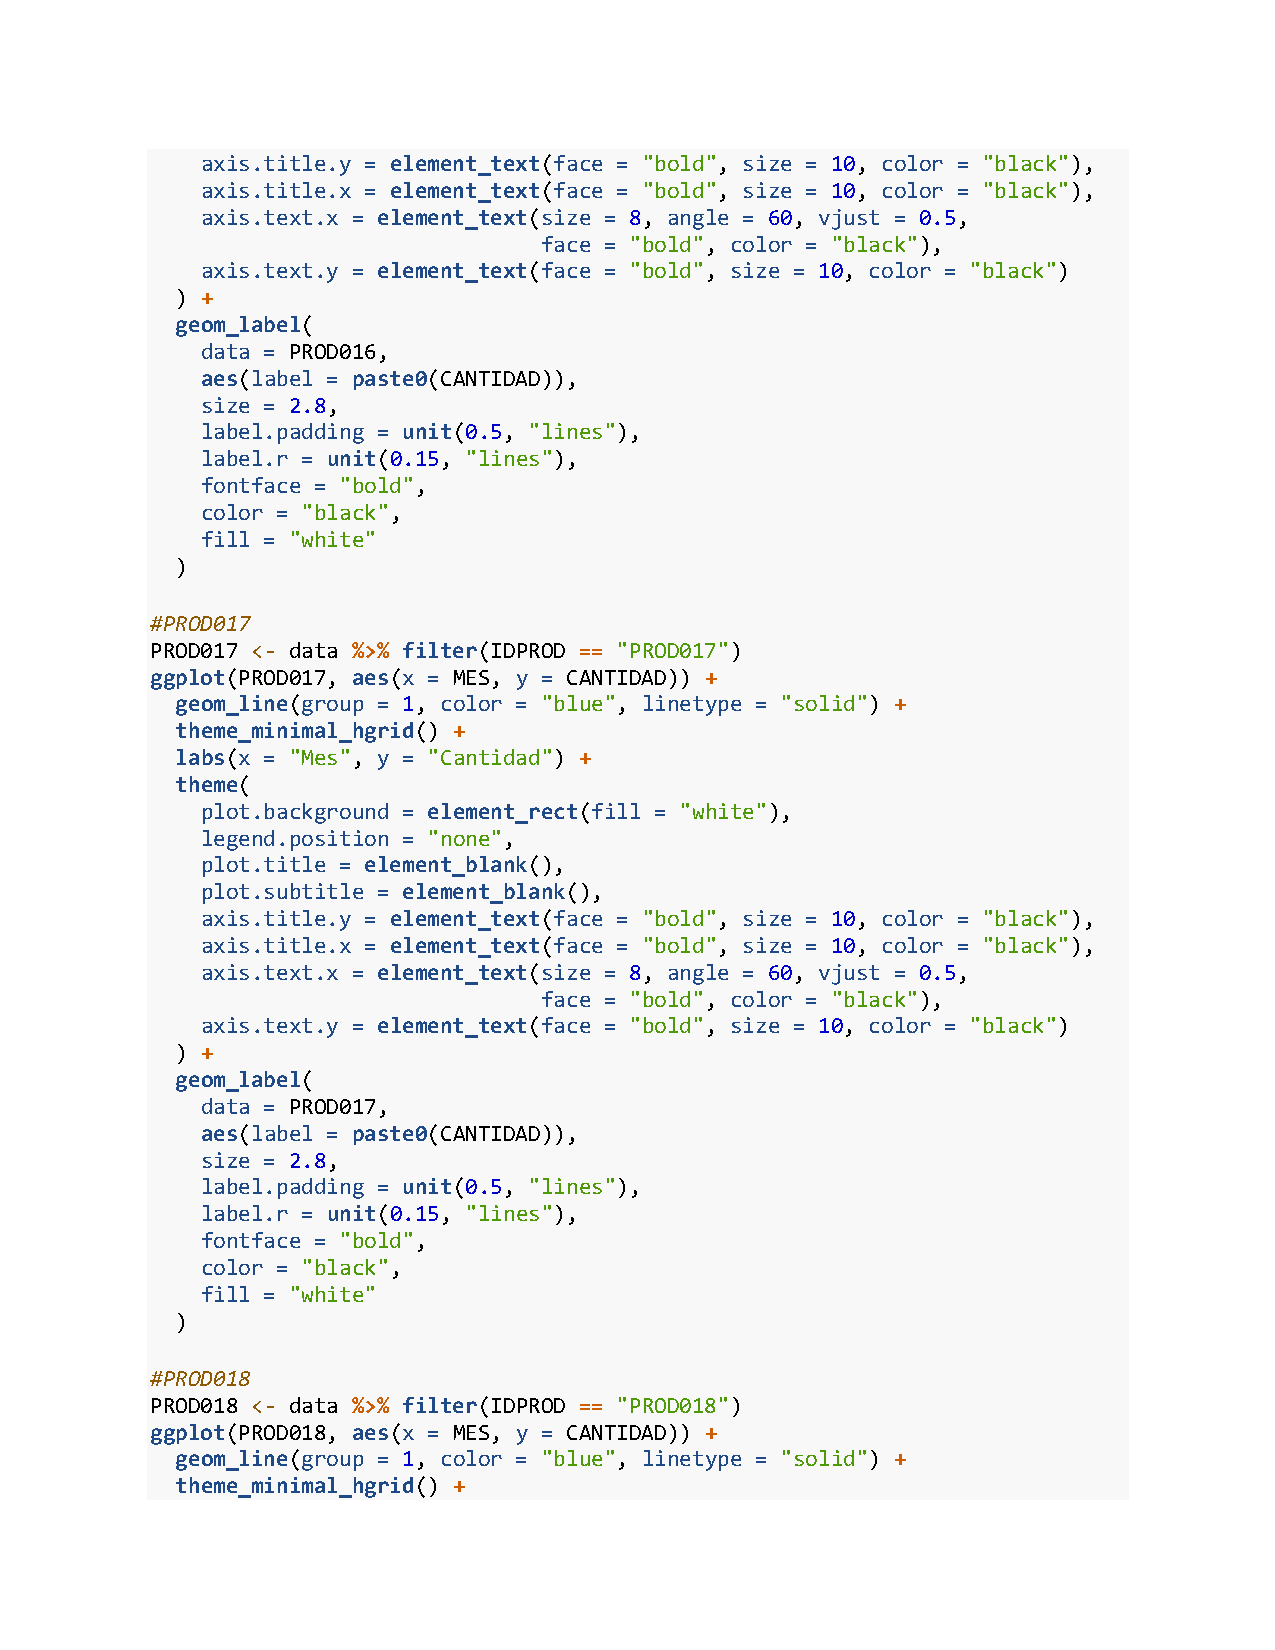
\includegraphics[width=\linewidth, height=22cm, trim=2.5cm 2.5cm 2.5cm 2.5cm, clip]{images/script15.pdf}}
        \end{tcolorbox}
\end{figure}

\begin{figure}[h!]
        \begin{tcolorbox}[colback=white, colframe=black, boxrule=1.5pt, sharp corners=all]
            {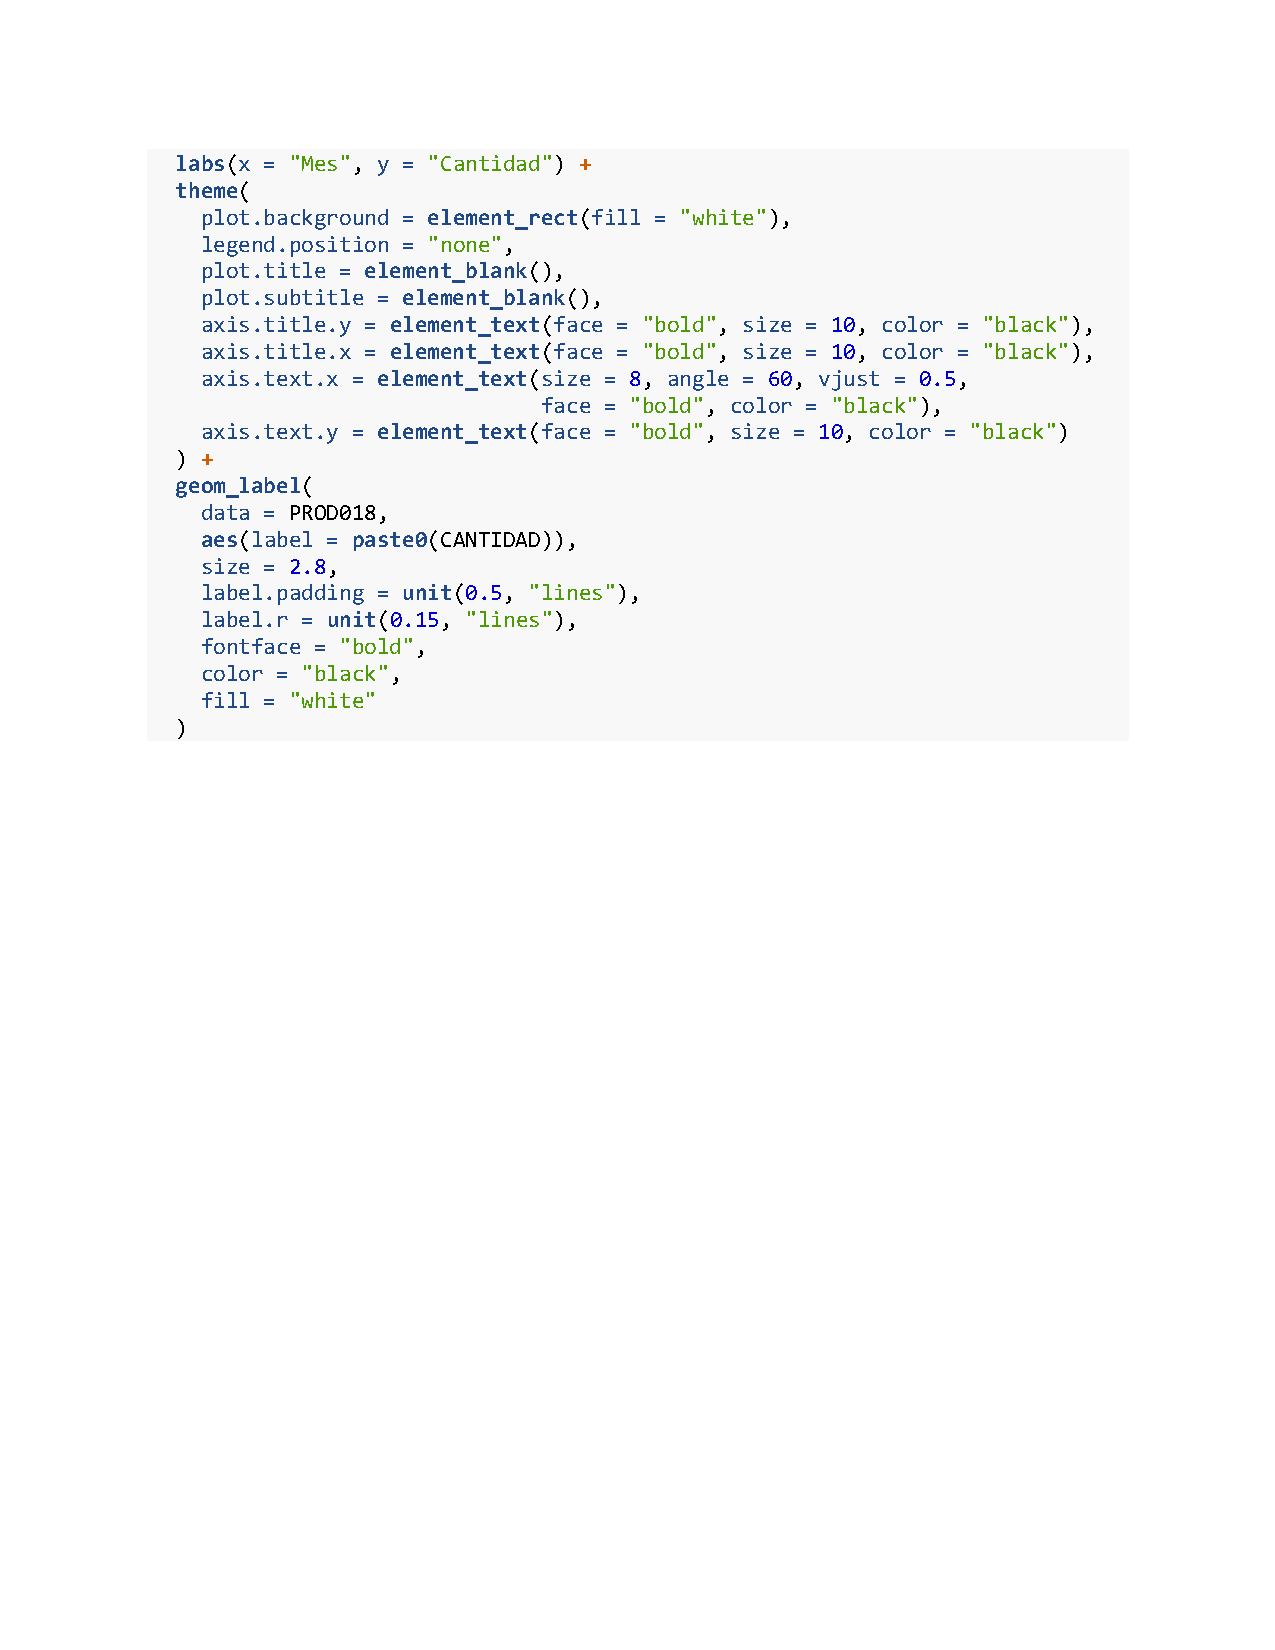
\includegraphics[width=\linewidth, height=22cm, trim=2.5cm 2.75cm 2.5cm 2.5cm, clip]{images/script16.pdf}}
        \end{tcolorbox}
\end{figure}

\clearpage
\begin{landscape}
\section{Base de datos}
\begin{figure}[h!]
  {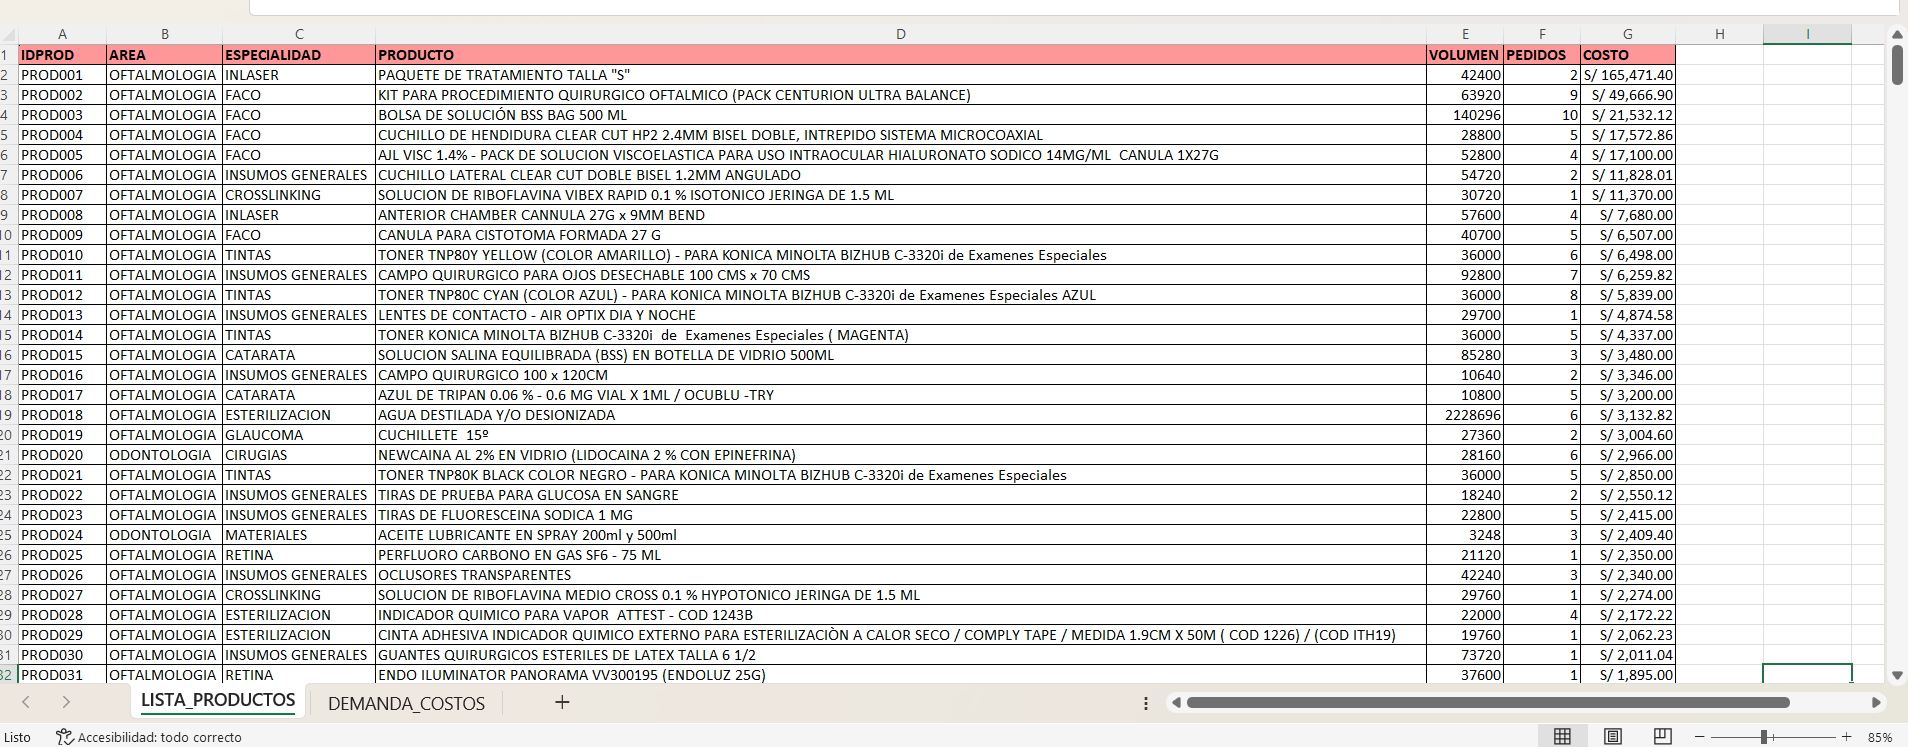
\includegraphics[width=24cm, height=14cm]{images/datos1.png}}
\end{figure}

\begin{figure}[h!]
  {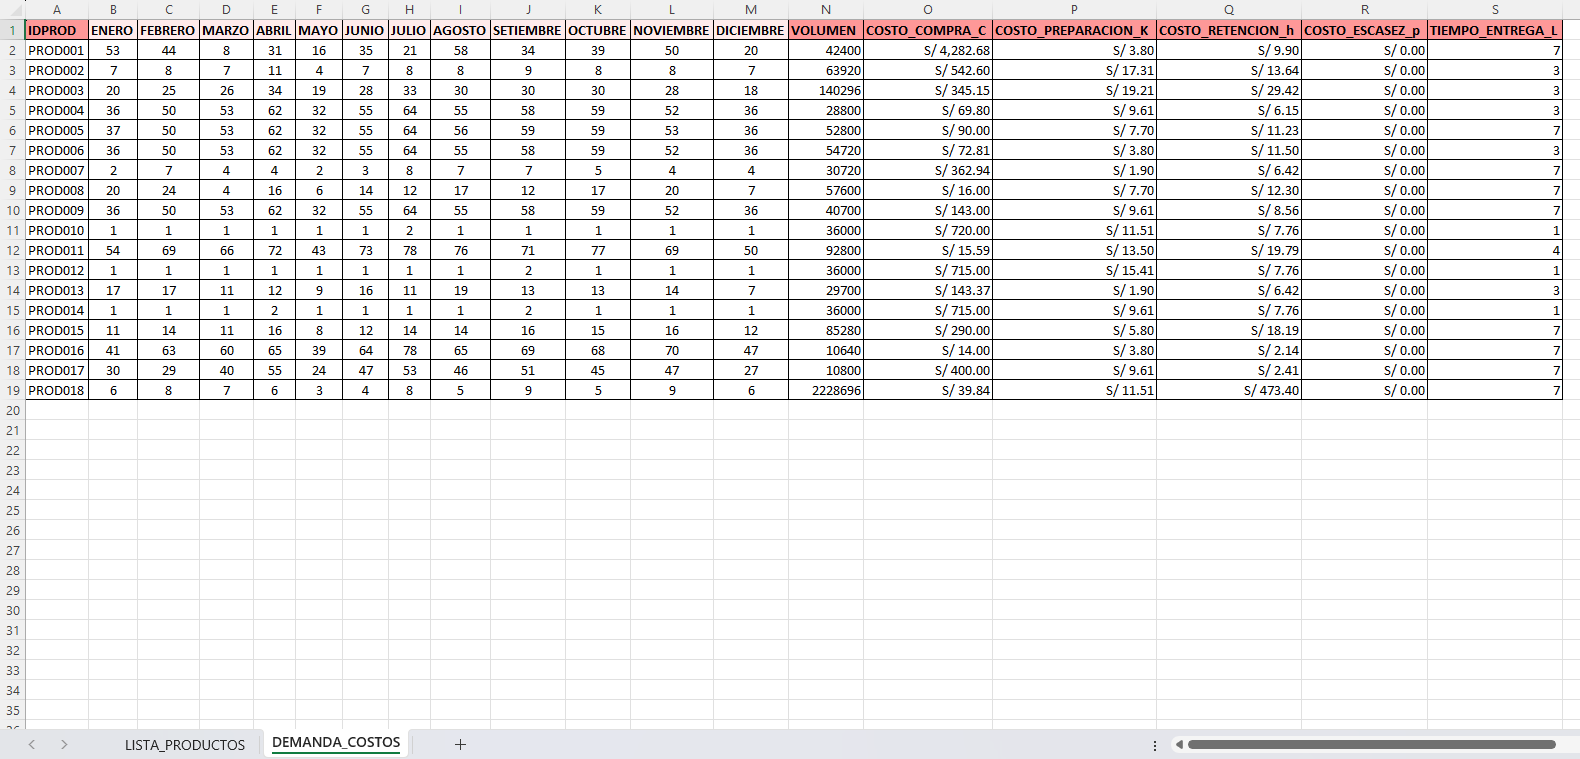
\includegraphics[width=24cm, height=15cm]{images/datos2.png}}
\end{figure}
\end{landscape}

%\addcontentsline{toc}{section}{B. Script código R}
%\textbf{B. Script código R}\\
%\lipsum[1-5]
%\textbf{Script Código R}

%\begin{figure*}[h]
%        \centering
%        \begin{tcolorbox}[colback=white, colframe=black, boxrule=1.5pt, sharp corners=all]
%            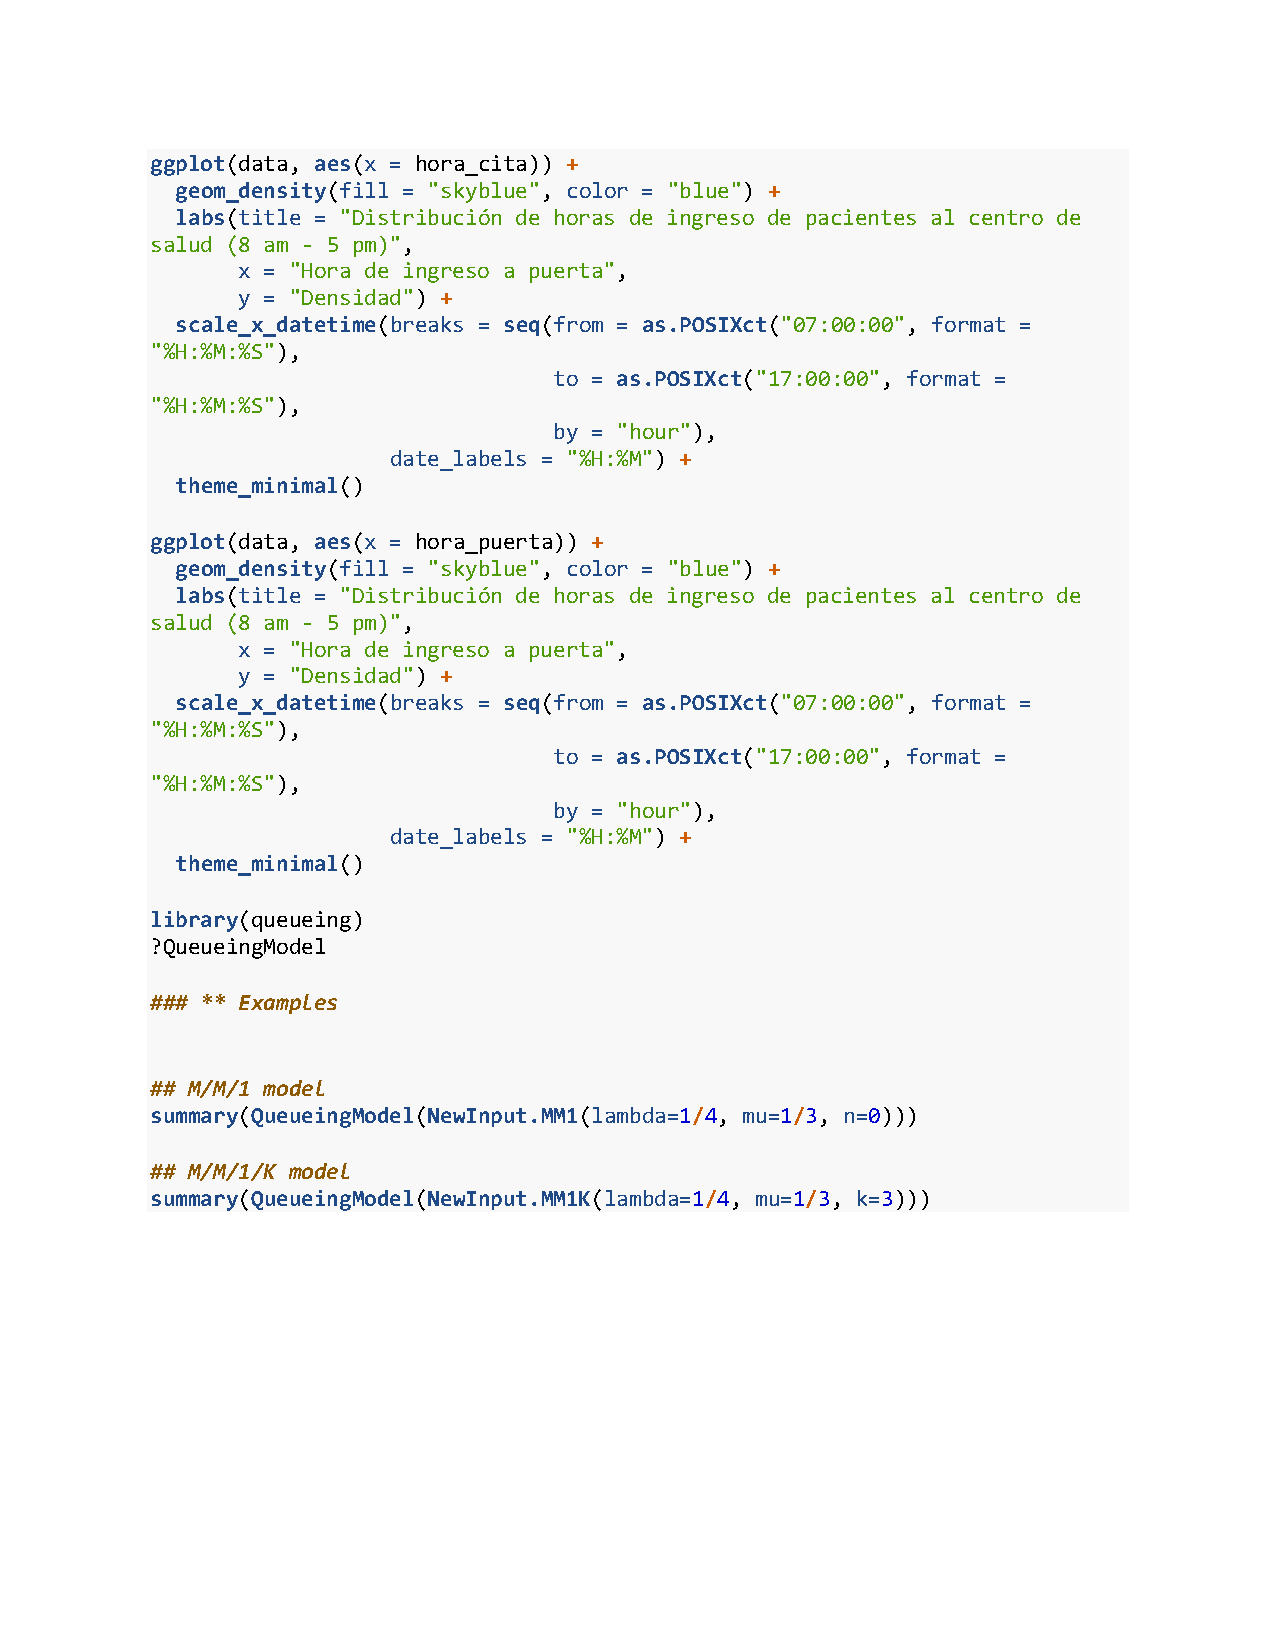
\includegraphics[width=\linewidth, height=15cm, trim=2.5cm 7cm 2.5cm 2.5cm, clip]{images/script_R.pdf}
%        \end{tcolorbox}
%    \end{figure*}
	
%\addcontentsline{toc}{section}{C. Otro imagenes}
%\textbf{C. Otro imagenes}\\
%\lipsum[1-5]

%\end{anexo}
